\documentclass[12pt]{article}
\usepackage[letterpaper, portrait, margin=1in]{geometry}
\usepackage{amsmath, amsthm, amssymb, physics, dsfont}
\usepackage{mathtools}

\usepackage{graphicx}
\graphicspath{/Users/darshanpatel/Desktop/LaTex Notes/Math390.4/}

\usepackage{fancyhdr}
\pagestyle{fancy}
\fancyhf{}
\lhead{Darshan Patel}
\rhead{Math 390.4: Data Science Basics}
\renewcommand{\footrulewidth}{0.4pt}
\cfoot{\thepage}

\begin{document}

\theoremstyle{definition}
\newtheorem{theorem}{Theorem}[section]
\newtheorem{definition}{Definition}[section]
\newtheorem{example}{Example}[section]

\newcommand{\set}[1]{\left\{ #1 \right\}}
\newcommand{\indicator}[1]{\mathds{1}_{#1}}
\newcommand{\argmin}[1]{\stackrel{\text{argmin}}{ #1 }}
\newcommand{\expe}[1]{\mathrm{E}[ #1 ]}
\renewcommand{\var}[1]{\mathrm{Var}[ #1 ]}
\newcommand{\prob}[1]{\mathbb{P}(#1)}
\newcommand{\cprob}[2]{\prob{#1~|~#2}}
\newcommand{\cov}[1]{\mathrm{Cov}[ #1 ]}
\newcommand{\corr}[1]{\mathrm{Corr}[ #1 ]}
\newcommand{\se}[1]{\mathrm{SE}[ #1 ]}
\newcommand{\reals}[1]{\mathbb{R}^{ #1 }}
\newcommand{\proj}[2]{\text{proj}_{ #1 } ( #2 )}
\newcommand{\projva}{\proj{\vec{v}}{\vec{a}}}
\newcommand{\colsp}[1]{\mathrm{colsp}\set{#1}}
\newcommand{\vhat}[1]{\vec{\hat{#1}}}
\newcommand{\nvec}[2]{\norm{\vec{#1}}^{#2}}
\newcommand{\vnorm}[1]{\norm{\vec{#1}}}
\renewcommand{\argmin}[1]{\stackrel{\text{argmin}}{#1}}
\newcommand{\argmax}[1]{\stackrel{\text{argmax}}{#1}}


\title{Math 390.4: Data Science Basics with Machine Learning and Statistical Modeling}
\author{Darshan Patel}
\date{Spring 2018}
\maketitle

\tableofcontents

\section{Lecture 1} 

\begin{definition} Models: abstractions/approximations to reality/ absolute truth/ system/ phenomenon \end{definition} 

Examples of Models: \begin{itemize} 
\item model airplane $\to$ airplane 
\item street map $\to$ city streets 
\item wind tunnel $\to$ airflow \end{itemize} 

``All models are wrong (not reality) but some are useful.'' -George Box. \\
Useful in the sense of providing predictions (what happened in a certain situation) and explanations (what makes the world tick?) \\
Data via simulation and data via direct measurement validate each other. \\
Why not just go with data via direct measurements? There is more control with simulations rather than in reality. 

\begin{definition} Validation: comparison of the measured data to the prediction; if they are ``close'', then the model is real; if not, we can rebuild the model, iterate and go closer. \end{definition} 

Model: ``Early to bed early to rise makes a man healthy, wealthy and wise.'" \\
Let's take this aphorism and see if it's a valid model. 
$$ \begin{bmatrix} \text{healthy} \\ \text{wealthy} \\ \text{wise} \end{bmatrix} = f(\text{bedtime, waketime})$$ 
The LHS is the output while the RHS is the inputs. \\
This model is ``imprecise;'' we need numbers and numerical measurements. \\~\\
Let's take our parameters and outputs to see if there is a way to acquire numerical measurements. 
 \begin{itemize} 
\item bedtime: average of $24$ hr time 
\item wake time: average of $24$ hr time 
\item health: longetivity 
\item wealth: net worth 
\item wisdom \end{itemize} 
Mathematical Model (MM) $\in$ Models \begin{itemize} 
\item MMs have numeric inputs and outputs 
\item MMs are related by an equal sign \end{itemize} 
Famous Examples: $$ \underbrace{F}_{\text{output}} = \underbrace{ma}_{2 \text{ inputs}} = f(m,a)$$
$$ E = mc^2 = f(m,c)$$ 
Let $y = t(z_1,z_2,\dots,z_t)$ where $y$ is output/ response/ outcome/ endpoint/ dependent variable, $(z_1,z_2,\dots, z_t)$ is ``true'' causal input information and $t$ is ``true'' relationship between the causal inputs and the output. \\~\\
An example of this relationship is with credit worthiness where $y \in \{ \text{creditworthy, uncreditworthy}\}$ or $y = \{0,1\}$ with $y$ being our output space. \\~\\
True Causal Inputs: \begin{itemize} 
\item $z_1$: has enough money at the time the loan is due $\in \{0,1\}$
\item $z_2$: unforeseen emergency $\in \{0,1\}$
\item $z_3$: criminal intent \end{itemize} 
Bigger Problem: $\{z_1,z_2,z_3\}$ are unobservable, not able to be measured, un-accessable, etc \\
Smaller Problem: don't know $t$ 

\section{Lecture 2} 
Recall $y \in \set{0,1} = Y$ \\
We had a true system (not a model but sometimes be ``the model.") $$y = t(z_1,z_2,z_3)$$ 
where $z_1 = $ has sufficient funds, $z_2 = $ unforeseen emergency and $z_3 = $ criminal intentions \\~\\
Problem: $\set{z_1,z_2,z_3}$ is unobserved (impossible to obtain). What to do? \\
Next best thing: Try to define and collect information ``related" to $\set{z_1,z_2,z_3}$ \\ 

Thus use what you have (or what is easily available). \\
Let's pretend we got the resources to ``define and collect." 
\begin{itemize} 
\item $x_1$: salary - measured by average salary
\item $x_2$: previous loan repayment - did they ever miss previous loan payment? $\in [0,1]$
\item $x_3$: historical criminal record - previous crime type? \\ $\set{\text{no crime}, \text{infraction}, \text{misdemeanor}, \text{felony}}$
\end{itemize} 

\begin{definition} Process Assessment: use as much as you got and whatever is cheaply available \end{definition}
Example: use age. \\~\\
Let's say we have $x_1,x_2,x_3$. The idea is $\set{z_1,z_2,z_3}$ which contains some info in $\set{x_1,x_2,x_3}$. \\ 

Let $\vec{x} = \begin{bmatrix} x_1 & x_2 & x_3 \end{bmatrix}$  where the LHS is an observation/ record/ object/ input/ independent variable and the RHS is features/ attributes/ characteristics/ regressors/ covariances/ predictors. \\
Note that $\dim{\vec{x}} = p$ or $d$.
$$ \vec{x} = \begin{bmatrix} x_1 & x_2 & x_3 \end{bmatrix} \in X $$ where $X$ is the covariance space. \\
Spaces: $x_1 \in \mathbb{R}$, $x_2 \in [0,1]$ - binary ordinary variable, $x_3$ - categorized variables with 4 ``levels" \\~\\
Two Ideas: \\
First to do: code is numerical, such as $x_3 \in \begin{bmatrix} 0 & 1 & 2 & 3 \end{bmatrix}$ - this should only be done if predictor is ``ordinal.'' \\
Next to do: Take $x_3$ and turn it into $x_{3a}$ (binary no crime), $x_{3b}$ - binary infraction, $x_{3c}$, $x_{3d}$. This increases $p$ from $3$ to $6$ - more variables to think about. \\
So, it is impossible to get $\set{z_1,z_2,z_3}$ but we do have $\begin{bmatrix} x_1 & x_2 & x_3 \end{bmatrix}$\\ 
GOAL: Do the best we can to explain $y$ by creating a model $f$, the approximation - the best relationship we can get. Does $y = f(x_1,x_2,x_3)$? No. \\
In fact, $$ \begin{aligned} y &\approx f(x_1,x_2,x_3) \\ y &= f(x_1, x_2,x_3) + \delta \end{aligned} $$ 
where $\delta = t(\vec{z}) - f(\vec{x})$, which comes from ignorance. \\
How do we get $f$? First note there is no analytical solution. \\
Example: $h(x) = x^2$. Find $\min{h}$. \\
Instead, use an ``empirical solution.'' An example of this is using data to learn from data. 
\begin{definition} Supervised Learning: uses historical examples of record and their responses \end{definition} 
In this case, it requires $3$ ingredients: 
$$ \mathcal{D} := \set{ \langle \vec{x}_1, y_1 \rangle, \langle \vec{x}_2, y_2 \rangle, \langle \vec{x}_3, y_3 \rangle} $$ 
where $\vec{x}_1$ is Bill's characteristics and $y_1$ is whether or not he paid back loan, $\vec{x}_2$ is Jill's, etc. \\
Let $$X = \begin{bmatrix} \vec{x}_1 \\ \vec{x}_2 \\ \vdots \\ \vec{x}_n \end{bmatrix} \in X^n,~~ Y = \begin{bmatrix} y_1 \\ y_2 \\ \vdots \\ y_n \end{bmatrix} \in Y^n $$ 
where $\dim(x) = n \cdot p$ and $\dim(\vec{y}) = n$.

\section{Lecture 3} 
Supervised Learning requires $3$ ingredients: \begin{enumerate} 
\item Training data - $$ \mathcal{D} := \set{ \langle \vec{x}_1, y_1 \rangle, \langle \vec{x}_2, y_2 \rangle, \dots, \langle \vec{x}_n, y_n \rangle} $$ There are historical input-output examples. $\vec{x}_1$ may be Bill's characteristics where $y_1 = 1$ (he paid his loan); $\vec{x}_2$ may be Jill's characteristics where $y_1 = 1$, etc. There are $n$ examples. Note: $\mathcal{D}$ is denoted using vector and matrix notation. $$ \mathcal{D} = \langle X, \vec{Y} \rangle $$ where $X \in \mathcal{X}^n \text{ if } \dim n \times p$ and $\vec{y} \in \mathcal{Y}^n = \set{0,1}^n$. 
\item $\mathcal{H} = \set{\text{all candidate functions } h \text{ that can approximate } f}$ This is needed because $f$ may be a very complicated function that can never be learned. So pick a large set of candidate functions that can approximate it. 
\item $\mathcal{A}$- an algorithm that takes in $\mathcal{D},\mathcal{H}$ and selects one best candidate function $g$ $$g = \mathcal{A}(\mathcal{D},\mathcal{H})$$ \end{enumerate} 

Review: $$y = t(z_1,\dots,z_t)$$ where $y$ is the phenomenon you wish to explain so you can predict in the future, $t$ is the true relationship that produces the phenomenon and $z_1,\dots,z_t$ is the causal attributes about the object that will produce the phenomenon. \\ 
$z_1,\dots, z_t$ are unobservable but $x_1,\dots,x_p$ are observable. 
$$ t = f(x_1,\dots,x_p) + \delta$$ where $$\delta = t(\vec{z}) - f(\vec{x})$$ $f$ is the best possible relationship given attributes you can measure and $\delta$ is the difference between the true relationship and the ``best we can do" (error due to ignorance). \\~\\
Goal: Estimate $f$. \\
You happen to have historical data $\mathcal{D}$ consisting of a prior examples. You have a finite space $\mathcal{H}$ of functions to approximate $f$ and an algorithm $\mathcal{A}$. You now use $\mathcal{A}$ to produce $g$. \\
If $f \in \mathcal{H}$, $$y = g(x_1,x_2,\dots,x_p) + \underbrace{(t(\vec{z}) - f(\vec{x}))}_{\text{error due to ignorance}} + \underbrace{(f(\vec{x}) - g(\vec{x}))}_{\text{parameter estimator error}} $$ 
The usual case: $f \notin \mathcal{H}$; this means there is a ``closest" function $h* \in \mathcal{H}$ but due to random chance, we pick $g$ instead. 
$$y = g(\vec{x}) + \underbrace{(t(\vec{z}) - f(\vec{x}))}_{\text{error due to ignorance}} + \underbrace{(f(\vec{x}) - h^*(\vec{x}))}_{\underbrace{\text{model misprediction}}_{f \notin \mathcal{H}}} + \underbrace{(h^*(\vec{x}) - g(\vec{x}))}_{\underbrace{\text{parameter estimator error}}_{g \neq h^*}} $$ 
There are $3$ sources of error. 

\section{Lecture 4} 

For supervised learning, you need $\mathcal{D}, \mathcal{H}, \mathcal{A}$ where $g = \mathcal{A}(\mathcal{D}, \mathcal{H})$. \\
How to get prediction? Let $\mathcal{D} = \set{\langle \vec{x}_i, y_i \rangle}$ where $ i - 1, \dots, n$. Your estimate is $\hat{y}_i = g(\vec{x}_i)$. It is also called an in-sample fit. \\ 
We want $\set{\hat{y}_1, \dots, \hat{y}_n}$, a set of in-sample fits / predictions to be $\approx \set{y_1,\dots, y_n}$, which is good but impossible due to 3 errors. \\
How to predict for new data/observation $\vec{x}^*$? Let $\hat{y}^* = g(\vec{x}^*)$. \\~\\
Let $y \in \set{0,1}$. Let's use only $x$ = salary. Then $$\mathcal{H} = \set{ \indicator{x > x_T}: x_T \in \mathbb{R}}$$, a family of step functions with a break at $x_T$, the parameter or threshold. \\ A more flexible model family to use is where there are multiple floor and ceiling functions put together on $\mathbb{R}$; however this is more complicated. Also, we still need $\mathcal{A}$, an algorithm. \\~\\
Let's define some error functions $\text{Err}(\vec{y}, \vec{\hat{y}}) > 0 \forall $ inputs. 
\begin{itemize} 
\item Mean of absolute error: $MAE = \frac{1}{n}\sum_{i=1}^n \abs{y_i - \hat{y}_i}$ \\
This is also called misclassification error and can be written as $\frac{1}{n} \sum_{i=1}^n \indicator{y_i \neq \hat{y}_i}$ 
\item Sum of absolute error: $SAE = \sum_{i=1}^n \abs{y_i - \hat{y}_i}$ 
\item Sum of squared error: $SSE = \sum_{i=1}^n (y_i - \hat{y}_i)^2$ 
\item Mean of squared error: $MSE = \frac{1}{n} \sum_{i=1}^n (y_i - \hat{y}_i)^2$ \end{itemize} 
Let $$SSE = \sum_{i = 1}^n (y_i - h(\vec{x}_i)) = \argmin{h \in \mathcal{H}} \set{SSE(h)} $$ 
This is the same as saying $$ x_T^* = \argmin{x_T} \set{ \sum_{i=1}^n (y_i - \indicator{\vec{x}_T - x_T})^2}$$ In this case, $\mathcal{A}$ would be a greedy search - tries every possibility. \\~\\
Let $X_1,X_2$ be continuous. Choose a model such that $$ \mathcal{H} = \set{ \indicator{x_1 > x_{T_1}}\indicator{x_2 > x_{T_2}} : \begin{bmatrix} x_1 \\ x_2 \end{bmatrix} \in \mathbb{R}^2 } $$ This would be a bad model because it would only capture values inside and outside a right angle. \\ A better model would be one that captures values above or below a certain line. $$ \begin{aligned} H &= \set{ \indicator{x_2 > a + bx_i : \begin{bmatrix} a \\ b \end{bmatrix} \in \mathbb{R}^2}} \\ &= \set{\indicator{a + bx_1 - x_2 > 0} : \begin{bmatrix} a \\ b \end{bmatrix} \in \mathbb{R}^2} \\ &= \set{\indicator{-a-bx_1 + x_2 > 0} : \begin{bmatrix} a \\ b \end{bmatrix} \in \mathbb{R}^2} \\ &= \set{\indicator{w_0 + w_1x_1 + w_2x_2 > 0}: \begin{bmatrix} w_0 \\ w_1 \\ w_2 \end{bmatrix} \in \mathbb{R}^3} \\ &= \set{\indicator{x_0 + \vec{w}\vec{x} > 0} : w_0 \in \mathbb{R}, \vec{w} \in \mathbb{R}^2} \end{aligned} $$ 
This is called a linear classifier. \\ 
Let $\vec{w} = \begin{bmatrix} 1 & x_1 & x_2 \end{bmatrix}$ where we augment $\vec{x}$ to include a $1$ in the first position, then we get $$ \mathcal{H} = \set{\indicator{\vec{w}\cdot \vec{x} > 0}: \vec{w} \in \mathbb{R}^3} $$ 
Use the same error function SSE 
$$g = \argmin{} \set{SSE(h)} \iff \vec{w}^* = \argmin{} \set{\sum_{i=1}^n (\indicator{\vec{w} \cdot \vec{x} > 0})^2} $$ 

\section{Lecture 5} 
Let $y = \set{0,1}$ and $X_1,\dots,X_n$ be the features. Then $$\mathcal{D} = \set{\begin{bmatrix} \vec{X}_1 \\ \vec{X}_2 \\ \vdots \\ \vec{X}_n \end{bmatrix}, \begin{bmatrix} y_1 \\ y_2 \\ \vdots \\ y_n \end{bmatrix}}$$
Note that we use $p+1$ because there is a bias of $1$ in our model. \\
We need $y^* = g(\vec{x}^*)$. Use $g = \mathcal{A}(\mathcal{H},\mathcal{D})$ where $$\mathcal{H} = \set{\indicator{\vec{w} \cdot \vec{x} > 0}, \vec{w} \in \mathbb{R}^{p+1}}$$ 
Perceptron Learning Algorithm: \begin{enumerate} 
\item Initialize $\vec{w}^{t = 0} = \vec{0}$ or random
\item Calculate $\hat{y}_i = \indicator{\vec{w}^t \cdot \vec{x} > 0}$
\item Update all weights from $j = 1,\dots,p+1$
$$ \begin{aligned} 
w_1^{t=1} &= w_1^{t = 0} + (y_i - \hat{y}_i)1 \\
w_2^{t=1} &= w_2^{t = 0} + (y_i - \hat{y}_i)x_{0,1} \\ 
&\vdots \\ 
w_{p+1}^{t = 1} &= w_{p+1}^{t = 0} + (y_i - \hat{y}_i)x_{p+1,1} \end{aligned} $$ 
\item Repeat steps $2$ and $3$ for all $i \in \set{1,\dots,n}$
\item Repeat steps $2$ through $4$ until a threshold error is reached or a maximum number of iterations. \end{enumerate} 
Note: If $\mathcal{D}$ is linearly separable ($\exists \vec{w}$ such that $\indicator{\vec{w} \cdot \vec{x} > 0}$) yields no errors in $\mathcal{D}$, then the algorithm will find it. \\~\\
Perceptron Diagrams: One Layer $$  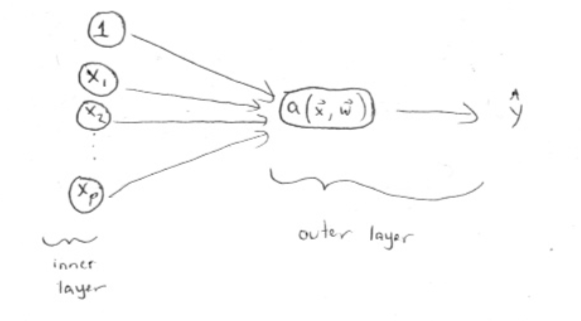
\includegraphics[scale = 0.7]{4c} $$
Two Layer $$ 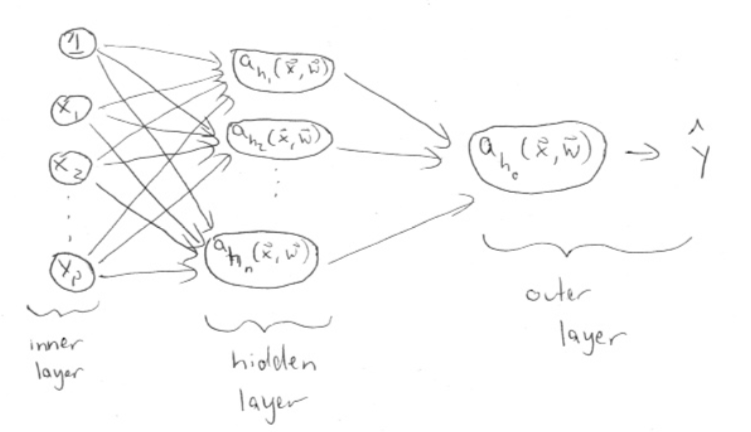
\includegraphics[scale = .5]{4d} $$ 

\section{Lecture 6} 
Null Model: a model where $\vec{x}$ does not matter; here, $\mathcal{H} = \set{0,1}$. Thus 
$$g = \mathcal{A}(\mathcal{D} = \vec{y}, \mathcal{H}) = \text{Mode}(\vec{y}) $$ 
Let $$ \mathcal{H} = \set{ \indicator{\vec{w} \cdot \vec{x} > 0} : \vec{w} \in \mathbb{R}^{p+1}}$$ Assume linear separability. Which hyperplane specified by $\vec{w}$ is the best? This would be the max-margin hyperplane, created by a wedge in between 2 lines separating data. This is called the Support Vector Machine (SVM) where SV is essential observations and M is model. Since data point $\vec{x}_i$ are ``vectors'', they are called the support vectors. \\
Let $$H = \set{\indicator{\vec{w} \cdot \vec{x} + b> 0}: w \in \mathbb{R}^p, b \in \mathbb{R}}$$
Example: Let $x_2 = 2x_1 + 2$. In the general equation of a line form, this is $$2x_1 - x_2 + 3 = 0 $$ 
To fit this into $\mathcal{H}$, we let $w = \begin{bmatrix} 2 \\ -1 \end{bmatrix}$, $x = \begin{bmatrix} x_1 \\ x_2 \end{bmatrix}$ and $b = 3$. Then $\vec{w} \cdot \vec{x} + b = 0$. Here $\vec{w}$ is a normal vector orthogonal to the line. \\~\\
Euclidean Norm: $\norm{\vec{w}} = \sqrt{ \sum_{j=1}^p w_i^2}$ - this is the length of the vector $\vec{w}$. \\
Normalized Vector $\vec{w}_0$: $\vec{w}_0 = \frac{\vec{w}}{\norm{\vec{w}}}$ - this is the vector $\vec{w}$ in the same direction but with length $1$. 
$$ \norm{\vec{w}_0} = \sqrt{ \sum_{j=1}^p \Big( \frac{w_j}{\norm{\vec{w}}} \Big)^2} = \sqrt{ \frac{1}{\norm{\vec{w}}^2} \sum_{j=1}^p w_j^2} = \sqrt{ \frac{1}{\norm{\vec{w}}^2} \norm{\vec{w}}^2} = 1 $$ 
Length of the line: $\vec{l} = \alpha \vec{w}_0$ where $\alpha \in \mathbb{R}$. 
$$ \norm{\vec{x}} = \sqrt{ \sum_{j=1}^p (\alpha w_{0j})^2} = \sqrt{ \alpha^2 \sum_{j=1}^p w_{0j}^2} = \sqrt{\alpha^2 \norm{\vec{w}_0}^2} = \abs{\alpha} $$ 
Let $\vec{l}$ be the vector from the origin to the line $\vec{w} \cdot \vec{x} + b = 0$, perpendicular to it. Solve for $\alpha$. Note that $\vec{l}$ is on the line $\vec{w} \cdot \vec{x} + b = 0$. 
$$ \begin{aligned} \vec{w} \cdot \vec{l} + b &= 0 \\ \vec{w} \cdot \alpha \vec{w}_0 + b &= 0 \\ 
\vec{w} \cdot \alpha \frac{ \vec{w}}{\norm{\vec{w}}} + b &= 0 \\ \alpha \frac{\norm{\vec{w}}^2}{\norm{\vec{w}}} + b &= 0 \\ \alpha &= - \frac{b}{\norm{\vec{w}}} \end{aligned} $$ Therefore 
$\abs{\alpha} = \frac{b}{\norm{\vec{w}}}$. \\
Going back the graph, we let the upper line be denoted as $\vec{w} \cdot \vec{x} + b + \delta = 0$ and the lower line as $\vec{w} \cdot \vec{x} + b - \delta = 0$. By this logic, the distance between the upper and lower lines is 
$$ \frac{b + \delta}{\norm{\vec{w}}} - \frac{b - \delta}{\norm{\vec{w}}} = \frac{2\delta}{\norm{\vec{w}}} $$ Since $c(\vec{w} \cdot \vec{x} + b) = 0$, there are infinite solutions because $c \in \mathbb{R}$. If we let $\delta = 1$, then we can find a unique solution to the equation, namely, $\frac{2}{\norm{\vec{w}}}$. \\
Constrain all $y = 1$s to be above the upper line and all $y = 0$s to be below the lower line. 
Then we find that $$ \begin{aligned} \vec{w} \cdot \vec{x} + b + 1 &\geq 0 \\ \vec{w} \cdot \vec{x} + b &\geq -1 \\ \forall i \text{ such that } y_i &= 1 \\ \vec{w} \cdot \vec{x}_i + b &\geq -1 \\ (y_i - \frac{1}{2})(\vec{w} \cdot \vec{x}_i + b) &\geq -(y_i - \frac{1}{2}) \\ \text{Since } y_i &= 1 \\ (y_i - \frac{1}{2})(\vec{w} \cdot \vec{x}_i + b) &\geq -(1 - \frac{1}{2}) \\ (y_i - \frac{1}{2})(\vec{w} \cdot \vec{x}_i + b) &\geq -\frac{1}{2} \end{aligned} $$ 
Now for all $i$ such that $y_i = 0$, $$ \begin{aligned} 
\vec{w} \cdot \vec{x}_i + b - 1 &\geq 0 \\ \vec{w} \cdot \vec{x}_i + b &= 1 \\ (y_i - \frac{1}{2})(\vec{w} \cdot \vec{x}_i + b) &\geq (y_i - \frac{1}{2}) \\ \text{Since } y_1 &= 0 \\ 
(y_i - \frac{1}{2})(\vec{w} \cdot \vec{x}_i + b) &\geq -\frac{1}{2} \end{aligned} $$ 
This is the condition of perfect separability. \\
To maximize $\frac{2}{\norm{\vec{w}}}$, we want to minimize $\norm{\vec{w}}$ subject to for all $i$, $(y_i - \frac{1}{2})(\vec{w} \cdot \vec{x}_i + b) \geq -\frac{1}{2}$ over $\vec{w} \in \mathbb{R}^p$ and $b \in \mathbb{R}$. The $\set{\vec{w}, b}$ solution is the SVM solution. This approach assumes perfect linear separability. In the real world, we do not always get that. We need a better $\mathcal{A}$. \\~\\
Let $SAE = \sum_{j = 1}^n \indicator{\hat{y}_i \neq y_i}$. Let's make a loss function dependent on how bad the error is. Consider the following: 
$$H_i = \max \set{0, -\frac{1}{2} - (y_i - \frac{1}{2})(\vec{w} \cdot \vec{x}_i + b)}$$ This is called the hinge loss. \\ 
Imagine the point is correctly classified and that it obeys the inequality. Consider it is above the inequality by $d \geq 0$. Then 
$$ (y_i - \frac{1}{2})(\vec{w} \cdot \vec{x}_i + b) = - \frac{1}{2} + d \geq -\frac{1}{2}$$ 
This is correct and so $$ H_i = \max \set{0, -\frac{1}{2} - (-\frac{1}{2} + d)} = \max \set{0,-d} = 0 $$ 
This makes sense because if it is correctly classified, then there should be zero error. \\
Imagine the point is incorrectly classified and hence does not obey the inequality. Consider it is below the inequality by $d > 0$. Then 
$$ (y_i - \frac{1}{2})(\vec{w} \cdot \vec{x}_i + b) = -\frac{1}{2} - d < -\frac{1}{2}$$ 
This is incorrect but 
$$ H_i = \max \set{0, -\frac{1}{2} - (-\frac{1}{2} - d)} = \max \set{0,d} = d > 0 $$ 
This makes sense; a mistake was made. \\~\\
Minimize $$\frac{1}{n} \sum_{i=1}^n H_i + \alpha + \norm{\vec{w}}^2 $$ 
This is the same as 
$$ \underbrace{\frac{1}{n} \sum_{i = 1}^n \max \set{0, -\frac{1}{2} - (y_i - \frac{1}{2})(\vec{w} \cdot \vec{x}_i + b)}}_{\text{min. avg. hinge loss}} + \underbrace{\lambda \norm{\vec{w}}^2}_{\text{max margin}} $$ 
This is our objective/loss function and it is a tradeoff between two goals. The parameters are $w \in \mathbb{R}^p$ and $b \in \mathbb{R}$. Therefore we still have $p + 1$ parameters. What is $\lambda$? It is a predefined constant called a ``hyperparameter." I is considered a tuning knob on the $\mathcal{A}$ itself. Recall $g(\vec{x}) = \indicator{\vec{w} \cdot \vec{x} + b}$. There is no $\lambda$ here. In fact, $\lambda$ only affects which $g \in \mathcal{H}$ will be selected. \\
Note: Perceptron algorithm does not work if not linearly separable! \\~\\
If $\lambda \approx 0$, we only care about errors and not a max margin. One error far away can ruin the nice separation line. If $\lambda \approx \infty$, we only care about the best line of separation and not about errors. This makes no sense. \\
Considering $\lambda$ is picked reasonably, how do we solve for $\set{\vec{w}, b}$? Use modern numerical optimization methods: quadratic programming, sub-gradient descent, coordinate descent, etc. 

\section{Lecture 7} 
Let $g = \mathcal{A}(\mathcal{D},\mathcal{H})$. Predict $\hat{y}^* = g(\vec{x}^*)$. What if $g$ found the closest $\vec{x}_i \in \mathcal{D}$ to $\vec{x}^*$ and returned $\hat{y}^* = y_i$? This closest $\vec{x}_i$ is called its neighbor. By closest, we need a notion of a difference between two observations:  
$$d(\vec{x}_i \vec{x}_k) = \norm{\vec{x}_i - \vec{x}_k}^2 = (\vec{x}_i - \vec{x}_k)^T(\vec{x}_i - \vec{x}_k) = \sum_{j=1}^p (x_{ij} - x_{kj})^2 $$ 
This is called $L1$ distance or Euclidean norm squared distance. Here, $\mathcal{H}$ and $\mathcal{A}$ are difficult to define. \\
What if $g$ located the closest $\vec{x}_i$?. Then $\hat{y} = \text{Mode}[y_1, \dots, y_k]$ where each $y_i$ represents the nearest $x_i$'s. This is called the $K$ nearest neighbors, or $KNN$ algorithm . The weakness of this algorithm is when $p$ is large, where there are too many dimensions and so not all $x_j$ terms are equally predictive. In this algorithm, $k$ and $d$ must be chosen. \\~\\ 
So far, we have only been concerned with $y = \set{0,1}$. This is called ``binary classification." Tif $y = \set{0,1,\dots, k}$, where the response level are nominal (no order), there is called ``classification" or ``multi-level classification." \\
What if $y \in \mathbb{R}$ or $y \in R \subseteq \mathbb{R}$? This is called ``regression." The threshold, perception and SVM cannot do regression without some adaptations. \\~\\
Null Model: doesn't care about $\vec{x}_i$s. Therefore $g(\vec{x}) = \overline{y} = \frac{1}{n} \sum_i y_i$. \\
Linear Regression Model: Consider $\mathcal{H} = \set{ \vec{w} \cdot \vec{x}: \vec{w} \in \mathbb{R}^{p+1}}$ where $\vec{x} = \begin{bmatrix} 1 & x_1 & \dots & x_p \end{bmatrix}$ and $\vec{w} = \begin{bmatrix} w_0 & w_1 & \dots & w_p \end{bmatrix}$. 
Then we get $$ H = \set{w_0 + w_1x_1 + \dots + w_px_p: w_0 \in \mathbb{R}, w_1 \in \mathbb{R}, \dots, w_p \in \mathbb{R}}$$ Here $\vec{w}$ is the linear coefficients. The dimension of this parameter space is $p+1$. \\
Imagine this for for $p = 1$ care. $$\mathcal{H} = \set{w_0 + w_1x_1: w_0 \in \mathbb{R}, w_1 \in \mathbb{R}}$$ Then the candidate in $\mathcal{H}$ that most closely resembles $f$ is $$ h^*(\vec{x}) = w_0^* + w_1^* = \beta_0 + \beta_1x $$ 
What about the errors? 
$$ y = h^*(\vec{x}) + \varepsilon = h^*(\vec{x}) + \overbrace{(t(\vec{z}) - f(\vec{x}))}^{\text{ignorance}} + \underbrace{(f(\vec{x}) - h^*(\vec{x}))}_{\text{misspecification of linear model}} $$ 
where $\varepsilon$ is the noise or error. Note that $h^*$ is inaccessible since we have to make an imperfect fit with finite data. Therefore 
$$ y = g(\vec{x}) + e = g(\vec{x}) + \underbrace{(t(\vec{z}) - f(\vec{x})) + (f(\vec{x}) - h^*(\vec{x}))}_\varepsilon + \overbrace{(h^*(\vec{x}) - g(\vec{x}))}^{e - \varepsilon} $$ 
where $e - \varepsilon$ is the estimation error. We call $e$ the residuals. \\
As $n \to \infty$, $g(\vec{x}) \to h^*(\vec{x})$ and $e - \varepsilon \to 0$. But $y \neq g(\vec{x})$ since the other two errors are still present. \\~\\
For the linear model for $p=1$, we need a loss function to fit $\vec{w}$. Recall the sum of squared error formula. Let's do some manipulations to it. $$ \begin{aligned} 
SSE &= \sum_{i=1}^n (y_i - \hat{y}_i)^2 = \sum e_i^2 \\ &= \sum_{i=1}^n (y_i - (w_0 + w_1x_i))^2 \\ &= \sum_{i=1}^n y_i^2 + w_0^2 + w_1^2x_i^2 - 2y_iw_0 - 2y_iw_1x_i + 2w_0w_1x_i \\ &= \sum y_i^2 + nw_0^2 + w_1^2\sum x_i^2 - 2n\overline{y}w_0 - 2w_1\sum x_iy_i + 2w_0w_1n\overline{x} \end{aligned} $$ 
Choose $w_0$ and $w_1$ to minimize the above. 
$$ \frac{\partial}{\partial w_0} SSE = 2nw_0 - 2n\overline{y} + 2w_1n\overline{x} = 0 \to \hat{w}_0 = \overline{y} - w_1\overline{x} $$ 
$$ \begin{aligned} \frac{\partial}{\partial w_1} SSE &= 2w_2 \sum x_i^2 - 2\sum y_ix_i + 2w_0n\overline{x} = 0 \\ &= w_1\sum x_i^2 - \sum y_ix_i + (\overline{y} - w_1\overline{x})n\overline{x} = 0 \\ 
&= w_1\sum x_i^2- \sum y_ix_i + n\overline{x}\overline{y} - w_1n\overline{x}^2 = 0 \\ 
w_1(\sum x_i^2 - n\overline{x}^2) &= \sum y_ix_i - n\overline{x}\overline{y} \\
\hat{w}_1 &= \frac{\sum y_ix_i - n\overline{x}\overline{y}}{\sum x_i^2 - n\overline{x}^2} = \frac{(n-1)S_{xy}}{(n-1)S_x^2} = r\frac{S_y}{S_x} \\ \hat{w}_0 &= \overline{y} - r\frac{S_y}{S_x}\overline{x} = \beta_0 \end{aligned} $$

\section{Lecture 8} 
Let $p = 1$ and $\mathcal{D} = \set{\begin{bmatrix} x_{11} \\ x_{21} \\ \vdots \\ x_{n1} \end{bmatrix}, \begin{bmatrix} y_1 \\ y_2 \\ \vdots \\ y_n \end{bmatrix}}$ where $\mathcal{Y} \in \mathbb{R}$. We want to create a $g$ for prediction using regression since $\mathcal{y} \subset \mathbb{R}$, not $\set{0,1}$. We want to classify $\hat{y} = g(x^*)$. Let 
$$H = \set{ \vec{w} \cdot \vec{x}: w \in \mathbb{R}^{p+1}} = \set{w_0 + w_1x: w_0 \in \mathbb{R}, w_1 \in \mathbb{R}}$$ 
Let $g = \mathcal{A}(\mathcal{D},\mathcal{H})$. Find an $\mathcal{A}$ that'll fit the two parameters $w_0$ and $w_1$. \\
Let $\mathcal{A}$ be ordinary least square regression. This requires solving the following problem:
$$ \begin{bmatrix} b_0 \\ b_1 \end{bmatrix} = \argmin{w_0,w_1} \set{SSE} = \sum_{i=1}^n (y_i - g(x_i))^2 = \sum_{i=1}^n (y_i - \hat{y}_i)^2 = \sum_{i=1}^n (y_i - (w_0 + w_1x_i))^2 = \sum_{i=1}^n e_i^2 $$ 
We call these least square estimates $b_0$ and $b_1$ and can also be denoted as $\hat{\beta}_0$ and $\hat{\beta}_1$, respectively. \\
How well does the model predict? 
$$ \begin{aligned} SSE &= \sum_{i = 1}^n (y_i - (b_0 + b_1x_i))^2 &\text{ sum of squared error, units: } y^2 \\ MSE &= \frac{1}{n-2}\sum_{i=1}^n (y_i - (b_0 + b_2x_i))^2 &\text{ mean squared error, units: } y^2 \\ RMSE &= \sqrt{MSE} &\text{ root mean squared error, units: } y \end{aligned} $$ 
The RMSE expresses the corrected variance of the $e$'s. The RMSE is just like standard deviation and has the same units. It is common to report prediction error as RMSE. \\
Another well known metric is called $R^2$, or the proportion of sample variance explained. \\
Consider the null model. What is the SSE of this model? 
$$SSE_0 = \sum (y_i - \overline{y})^2 = (n-1)s_y^2 = SST \text{ sum of squared total} $$ 
After the model is fit, there is a new, hopefully lower SSE. 
$$SSE = \sum e_i^2 = (n-1)s^2_e $$ 
This means that the model has less error and variance is explained. \\
How much SSE/$s^2$ has been reduced as a proportion of the null SSE/$s^2$? 
$$ \begin{aligned} R^2 &= \frac{SSE_0 - SSE}{SSE_0} = \frac{s_y^2 - s_e^2}{s_y^2} \\
&= \frac{SST - SSE}{SST} \\ &= 1 - \frac{SSE}{SST} \\ &= SSR \end{aligned} $$ 
Furthermore, the proportion of sample variance explained is estimated as 
$$ \frac{s_y^2 - s_e^2}{s_y^2} = \frac{\var{Y} - \var{E}}{\var{Y}} $$ 
Sine $s^2 > 0$, then $R^2 \leq 1$. Can $R^2 < 0$? Yes. What about $s^2_e > s^2_y$? This means that the model is worse than the null model \\
Another way to see this is as follows: Let the null model be $g(x) = \overline{y}$. The residuals will be $e_i = y_i - \overline{y}$. Fit a simple linear regression model $g(x) = b_0 + b_1x$. Then the residuals will be $e_i = y_i - (b_0 + b_1x_i)$. This is a much narrower graph because $s^2_e$ dropped a lot. \\
RMSE vs. $R^2$: Which is more important for assessing predictive ability? RMSE. It answers how good the predictions are and the standard deviation of the predictions. \\
As $R^2$ increases, RMSE decreases. As $R^2$ decreases, RMSE increases. \\
If $R^2 = 99\%$, the RMSE could still be big. Maybe there was a ton of variance in $y$. You explained most of it but there is still a lot left. 
$$RMSE \approx s_e $$ 
Empirical Rule: $\hat{y} \pm 2\cdot s_e \approx 95\%$ of all predictions (if $E \sim N(0,\sigma^2)$). Also, $\hat{y} \pm 3\cdot s_e \approx 99.7\%$ of all predictions. 

\section{Lecture 9} 
What if you're doing regression $\mathcal{y} \subseteq \mathbb{R}$ and $p = 1$ but the feature is a factor with two levels. Let $x = \mathcal{X} = \set{\text{red, green}}$. How do you model this? Try linear model. \\
Let red be represented as $0$ and green as $1$. Create a binary variable $\tilde{x} \in \set{0,1}$. What would the hyper set look like? 
$$ \mathcal{H} = \set{w_0 + w_1\tilde{x}: w_0 \in \mathbb{R}, w_1 \in \mathbb{R}} = \set{w_0 + w_1\indicator{x = \text{green}}: w_0 \in \mathbb{R}, w_1 \in \mathbb{R}} $$ 
Therefore the final model is $$\hat{y} = b_0 + b_1\tilde{x} = b_0 + b_1\indicator{x = \text{green}} $$ 
This model can be fitted with least squares. 
$$\hat{y} = \begin{cases} \bar{y}_{\text{red}} &\text{ if } x = \text{ red} \\ \bar{y}_{\text{green}} &\text{ if } x = \text{ green} \end{cases} = \underbrace{\bar{y}_{\text{red}}}_{b_0} + \underbrace{(\overbrace{\bar{y}_{\text{green}} - \bar{y}_{\text{red}}}^{\Delta \bar{y}})}_{b_1}\indicator{x = \text{ green}} $$ 
Red is called the reference level/category and thus $b_1$ represents the added effect of green over red. \\
Proof: Let $p = \frac{1}{n}\sum \indicator{x_1 = \text{ green}}$ (the proportion of greens); therefore $1-p$ is the proportion of red. Let $b_0 = \bar{y} - b_1\bar{x}$ and assume $b_1 = \bar{y}_g - \bar{y}_r$. Then 
$$\bar{y} = \frac{y_1 + \dots + y_n}{n} = \overbrace{\frac{y_{1g} + \dots + y_{ng}}{n}}^{\text{greens}} + \overbrace{\frac{y_{1r} + \dots + y_{nr}}{n}}^{\text{reds}} = \frac{\bar{y}_gn_g}{n} + \frac{\bar{y}_rn_r}{n} = \bar{y}_g\frac{n_g}{n} + \bar{y}_r\frac{n_r}{n}$$
Let $\bar{x} = \frac{x_1 + \dots + x_n}{n} = \frac{x_{g1} + \dots x_{gn} + x_{r1} + \dots + x_{rn}}{n} = \frac{n_g}{n} = p$. Then $$ \bar{y} = p\bar{y}_g + (1-p)\bar{y}_r $$ 
For $b_0$: 
$$ b_0 = p\bar{y}_g + (1-p)\bar{y}_r - p(\bar{y}_g - \bar{y}_r) = (1-p)\bar{y}_r + p\bar{y}_r = \bar{y}_r $$ 
Now for $b_1$, note first that
 $$ \begin{aligned} \sum x_iy_i &= \sum y_{gi} = ng\bar{y}_g \\ n\bar{x}\bar{y} &= np\bar{y} \\ \sum x_i^2 &= n_g \\ n\bar{x}^2 &= np^2 \end{aligned} $$ 
Then: 
$$ \begin{aligned} b_1 &= r\frac{s_y}{s_x} \\ &= \frac{\sum x_iy_i - n\bar{x}\bar{y}}{\sum x_i^2 - n\bar{x}^2} \\ &= \frac{n_g\bar{y}_g - np\bar{y}}{n_g - np^2} \cdot \frac{1/n}{1/n} \\ &= \frac{p\bar{y}_g - p\bar{y}}{p - p^2} \\ &= \frac{\bar{y}_g - \bar{y}}{1-p} \\ &= \frac{\bar{y}_g - (p\bar{y}_g + (1-p)\bar{y}_r)}{1-p} \\ &= \frac{\bar{y}_g}{1-p} - \frac{p\bar{y}_g}{1-p} - y_r \\ &= \bar{y}_g - \bar{y}_r \end{aligned} $$ 
This is a line connecting the means of green and red where the difference in $y$ is $\bar{y}_g - \bar{y}_r$. \\
What if there were more than $2$ levels in the function? For example, $x = \set{\text{red, green, blue}}$. Recall that $x$ can be rewritten as $\set{\tilde{x}_1, \tilde{x}_2, \tilde{x}_3}$. Here one variable becomes three (dummy) variables. 
$$ \begin{aligned} x_1 &= \indicator{x = \text{ red}} \\ x_2 &= \indicator{x = \text{ green}} \\ x_3 &= \indicator{x = \text{ blue}} \end{aligned} $$ 
We cannot use a model on $y \sim x$ here. This leads to multivariate linear regression. 

\section{Lecture 10} 
Random variables $X$ and $Y$ are said to be dependent if knowing the value of one affects the distribution of the other $$\cprob{Y}{X=x} \neq \prob{Y}$$ 
In data science terminology, if knowing a prediction $x$ allows you to know something about $y$, then $x$ and $y$ are associated. \\
Recall covariance: $$ \cov{X,Y} = \expe{(X - \mu_X)(Y - \mu_Y)}$$ which can be estimated by $$s_{xy} = \frac{1}{n-1}\sum (x_i - \bar{x})(y_i - \bar{y}) \in \mathbb{R}$$ 
Sign of the Covariance: if $x$ increases and $y$ increases, then covariance is positive; if $x$ increases and $y$ decreases, then covariance is negative. 
Recall: $$\rho = \corr{X,Y} = \frac{\cov{X,Y}}{\se{X}\se{Y}} \in [-1,1] $$ 
Correlation is estimated by $$r = \frac{s_{X,Y}}{s_Xs_Y} \in [-1,1] $$ 
Thus we say correlation is a standardized covariance. \\~\\
$X$,$Y$ are positively correlated if $r>0$ which means if $x$ increases, then $y$ increases. $X$,$Y$ are negatively correlated if $r<0$ which means if $x$ increases, then $y$ decreases. $X$, $Y$ are not correlated if $r=0$ which means if $x$ increases, then $y$ is unchanged. \\~\\
Let $\mathbb{Y} \subseteq \mathbb{R}$ where $p = 1$ and $\mathcal{H} = \set{\vec{w} \cdot \vec{x} = w_0 + w_1x: w_0 \in \mathbb{R}, w_1 \in \mathbb{R}}$. Now let $p=2$ and so $$\mathcal{H} = \set{w_0 + w_1x_1 + w_2x_2: \vec{w} \in \mathbb{R}^3} $$ 
For any $\vec{w}$, $$ SSE = \sum_{\langle \vec{x}_i, y_i \rangle \in \mathcal{D}} \overbrace{(y_i - (w_0 + w_1x_{i1} + w_2x_{i2}))^2}^{(y_i - \hat{y}_i)^2}$$ 
To solve for $\vec{w}$, take $$ \frac{\partial SSE}{\partial w_0} \stackrel{\text{set}}{=} 0, ~~~ \frac{\partial SSE}{\partial w_1} \stackrel{\text{set}}{=} 0, ~~~ \frac{\partial SSE}{\partial w_2} \stackrel{\text{set}}{=} 0 $$ 
There is a better method to figure out $\vec{w}$. \\
Let $\mathcal{D} = \langle X, \vec{y} \rangle$ where $$ X = \begin{bmatrix} 1 & X_{11} & X_{12} \\ 1 & X_{21} & X_{22} \\ \vdots & \vdots & \vdots \\ 1 & X_{n1} & X_{n2} \end{bmatrix} \in \mathbb{R}^{n\times p} = \mathbb{R}^{n\times 3} $$
Then $$ X\vec{w} = \begin{bmatrix} w_0 + w_1X_{11} + w_2X_{12} \\ w_0 + w_1X_{21} + w_2X_{22} \\ \vdots \\ w_0 + w_1X_{n1} + w_2X_{n2} \end{bmatrix} = \begin{bmatrix} \hat{y}_1 \\ \hat{y}_2 \\ \vdots \\ \hat{y}_n \end{bmatrix} $$
 This means $$\vec{\hat{y}} = X\vec{w}$$
Recall the following properties from linear algebra:  $$ \begin{aligned} (\vec{a} + \vec{b})^T &= \vec{a}^T + \vec{b}^T \\ \vec{a} \cdot \vec{b} &= \vec{b} \cdot \vec{a} \\ (AB)^T &= B^TA^T \\ \forall \vec{v} \in \mathbb{R}^d, ~ \vec{v} \cdot \vec{v} &= \sum_{j=1}^d v_j^2 = \vec{v}^T\vec{v} \end{aligned} $$ Then $$ \begin{aligned} 
SSE &= \sum_{i=1}^n (y_i - \hat{y}_i)^2 \\ &= (\vec{y} - \vec{\hat{y}})^T(\vec{y} - \vec{\hat{y}}) = (\vec{y}^T - \vec{\hat{y}}^T)(\vec{y} - \vec{\hat{y}}) \\ &= \vec{y}^T\vec{y} - \vec{\hat{y}}^T\vec{y} - \vec{y}^T\vec{\hat{y}} + \vec{\hat{y}}^T\vec{\hat{y}} \\ &= \vec{y}^t\vec{y} - 2\vec{\hat{y}}^T\vec{y} + \vec{\hat{y}}^T\vec{\hat{y}} \\ &= \vec{y}^T\vec{y} - 2(X\vec{w})^T\vec{y} + (X\vec{w})^T(X\vec{w}) \\ &= \vec{y}^T\vec{y} - 2\vec{w}^tX^T\vec{y} + \vec{w}^TX^TX\vec{w} \end{aligned} $$ 
Now take the partial derivative with respect to $\vec{w}$ and set it equal to $\vec{0}_{p+1}$ (vector derivative). 
$$ \frac{\partial SSE}{\partial \vec{w}} = \begin{bmatrix} \frac{\partial}{\partial w_0} SSE \\ \vdots \\ \frac{\partial}{\partial w_p} SSE \end{bmatrix} = \vec{0}_{p+1} $$ 
Properties: \begin{itemize}
\item For a constant $a \in \mathbb{R}$ and $\vec{c} \in \mathbb{R}^n$, $$ \frac{\partial}{\partial \vec{c}} a = \begin{bmatrix} \frac{\partial}{\partial c_1} a \\ \vdots \\ \frac{\partial}{\partial c_n} \end{bmatrix} = \vec{0}_n$$ 
\item For $\vec{c} \in \mathbb{R}^n$, $$ \begin{aligned} \frac{\partial}{\partial \vec{c}} (af(\vec{c}) + g(\vec{c})) &= \begin{bmatrix} \frac{\partial}{\partial c_1} (af(\vec{c}) + g(\vec{c})) \\ \vdots \\ \frac{\partial}{\partial c_n} (af(\vec{c}) + g(\vec{c})) \end{bmatrix} \\ 
&= \begin{bmatrix} a\frac{\partial}{\partial c_1} f(\vec{c}) + \frac{\partial}{\partial c_1} g(\vec{c}) \\ \vdots \\ a\frac{\partial}{\partial c_n} f(\vec{c}) + \frac{\partial}{\partial c_n} g(\vec{c}) \end{bmatrix} \\ 
&= a\frac{\partial}{\partial{\vec{c}}} f(\vec{c}) + \frac{\partial}{\partial \vec{c}} g(\vec{c}) \end{aligned} $$ 
\item For $\vec{c} \in \mathbb{R}^n$ and $\vec{b} \in \mathbb{R}^n$, 
$$ \frac{\partial}{\partial \vec{c}} ~\vec{c}^T\vec{b} = \frac{\partial}{\partial \vec{c}} (c_1b_1 + c_2b_2 + \dots + c_nb_n) = \begin{bmatrix} b_1 \\ \vdots \\ b_n \end{bmatrix} = \vec{b} $$ 
\item For $A \in \mathbb{R}^{n\times n}$ and $\vec{c} \in \mathbb{R}^n$ and $A$ symmetric, note first that $$ A\vec{c} = \begin{bmatrix} a_{11}c_1 + a_{12}c_2 + \dots + a_{1n}c_n \\ a_{21}c_1 + a_{22}c_2 + \dots + a_{2n}c_n \\ \vdots \\ a_{n1}c_1 +a_{n2} + \dots + a_{nn}c_n \end{bmatrix}$$ and that $$ \vec{c}^T(A\vec{c}) = c_1(a_{11}c_1 + a_{12}c_2 + \dots + a_{1n}c_n) + \dots + c_n(a_{n1}c_1 + a_{n2}c_2 + \dots + a_{nn}c_n) = \sum_{j=1}^n\sum_{i=1}^n a_{ij}c_ic_j$$
Then $$ \frac{\partial}{\partial \vec{c}}~ \vec{c}^T(A\vec{c}) = \begin{bmatrix} \frac{\partial}{\partial c_1} A\vec{c} \\ \vdots \\ \frac{\partial}{\partial c_n} A\vec{c} \end{bmatrix} = \begin{bmatrix} 2\vec{a}_{1\cdot}^T\vec{c} \\ \vdots \\ 2\vec{a}_{n\cdot}^T\vec{c} \end{bmatrix} = 2\begin{bmatrix} \vec{a}_{1\cdot} \\ \vdots \\ \vec{a}_{n\cdot} \end{bmatrix} \vec{c} = 2A\vec{c}$$ \end{itemize} 
Now let's apply this to SSE. 
$$ \begin{aligned} \frac{\partial}{\partial \vec{w}} SSE &= \frac{\partial}{\partial \vec{w}} (\vec{y}^T\vec{y} - 2\vec{w}^TX^T\vec{y} + \vec{w}^TX^TX\vec{w}) \\ &= \frac{\partial}{\partial \vec{w}} (\vec{y}^T\vec{y}) - 2\frac{\partial}{\partial \vec{w}} (\vec{w}^TX^T\vec{y}) + \frac{\partial}{\partial \vec{w}} (\vec{w}^TX^TX\vec{w}) \\ &= \vec{0} - 2X^T\vec{y} + 2X^TX\vec{w} \stackrel{\text{set}}{=} 0 \\ X^T\vec{y} &= X^TX\vec{w} \\ \vec{w} = \vec{b} &= (X^TX)^{-1}X^T\vec{y} \end{aligned} $$ 
Note that $X^TX$ is of dimension $\mathbb{R}^{p+1 \times p+1}$. It is invertible only when
$X^TX$ is of full rank $p+1$ (linearly independent), or rank($X$) = $p+1$. \\
Proof by Contradiction: Assume rank($X^TX) = p+1$ and rank($X) < p+1$. Then there is a non-trivial null space, meaning a vector $\vec{u} \neq \vec{0}$ and in $\mathbb{R}^{p+1}$ that can be mapped to $\vec{0}$. This means $X\vec{u} = \vec{0}_n$. But then if we use $X^TX$ to map vector $\vec{u}$, 
$$ (X^TX)\vec{u} = X^T(X\vec{u}) = X^T\vec{0}_n = \vec{0}_{p+1}$$ This means $\vec{u}$ is in the null space of $X^TX$. Therefore the dimension of the null space of $X^TX$ is greater than $0$. Then $X^TX$ is not full rank. Contradiction. \\~\\
When we say rank($X$) = $p+1$, we mean that each column is not linearly dependent on other columns. Therefore no predictive information is duplicated. \\
Henceforth, $$\vec{\hat{y}} = X\vec{b} = X(X^TX)^{-1}X^T\vec{y} = \vec{H}\vec{y}$$ 
where $\vec{H} = X(X^TX)^{-1}X^T$ is a hat matrix. 

\section{Lecture 11} 
Extrapolation: $$ x^* \notin \text{Range}[X] $$ 
where $$\text{Range}[X] = [X_{\cdot 1, \min}, X_{\cdot 1, \max}] \times [X_{\cdot 2, \min}, X_{\cdot 2, \max}] \times \dots \times [X_{\cdot p, \min}, X_{\cdot p, \max}] $$ 
each being the interval of the min and max of the $i$th prediction. \\~\\
Let $\vec{y} \in \mathbb{R}^n$ and $X \in \mathbb{R}^{n \times (p+1)}$. The linear multivariate least squares fitting is given by $$\vec{b} = (X^TX)^{-1}X^T\vec{y}$$ 
such that $$\vec{\hat{y}} = X\vec{b} = \begin{bmatrix} \leftarrow & \vec{X}_1 & \rightarrow \\ \leftarrow & \vec{X}_2 & \rightarrow \\ & \vdots & \\ \leftarrow & \vec{X}_n & \rightarrow \end{bmatrix} \vec{b} = X(X^TX)^{-1}X^T\vec{y} = H\vec{y}$$ 
The rank of $X$ is $p+1$ because $\hat{y}_i = b_0 + b_1x_{i1} + \dots + b_px_{ip}$ which lines in a $p+1$ dimension space. We call $p+1$ the degrees of freedom because it is the dimension of the column space of $X$. \\~\\
Recall that $\vec{y} = g(\vec{x}) + \vec{e} = \vec{\hat{y}} + \vec{e}$, Therefore $\vec{e} = \vec{y} - \vec{\hat{y}}$. $$SSE = \sum_{i=1}^n e_i^2 = \norm{\vec{e}}^2 $$ 
Furthermore, $$MSE = \frac{1}{n - (p+1)} = SSE $$ where $p+1$ is the degree of freedom. Then $$RMSE = \sqrt{MSE} = \sqrt{\frac{1}{n - (p+1)} SSE} = \frac{\norm{\vec{e}}}{\sqrt{n-(p+1)}} $$ 
Same as before, $$R^2 = \frac{S_y^2 - S_e^2}{S_y^2} $$ 
Orthogonal Projection: Project two vectors in $\mathbb{R}^d$ separated by an angle $\theta$ between a point joining it. By dropping $\vec{a}$ vertically down on $\vec{v}$, that is the $\text{proj}_{\vec{v}} (\vec{a})$. Its length will be called $l$. By the law of cosines, $$\cos \theta = \frac{\vec{a} \cdot \vec{c}}{\norm{\vec{a}} \norm{\vec{v}}} $$ 
Therefore $$ l = \norm{\vec{a}} \cos\theta = \frac{\vec{a} \cdot \vec{v}}{\norm{\vec{v}}} $$ Then $$ \text{proj}_{\vec{v}} (\vec{a}) = l \frac{\vec{v}}{\norm{\vec{v}}} = \frac{\vec{a} \cdot \vec{v}}{\norm{\vec{v}}^2} \vec{v} = \frac{\vec{a} \cdot \vec{v}}{\vec{v} \cdot \vec{v}} \vec{v} = \frac{\vec{v}\vec{v}^T\vec{a}}{\vec{v}^T\vec{v}} = \frac{\vec{v}\vec{v}^T}{\vec{v}^T\vec{v}} \vec{a} = H\vec{a} $$ Note that 
$$ HH = \Big( \frac{\vec{v} \cdot \vec{v}^T}{\norm{\vec{v}}^2}\Big)\Big( \frac{\vec{v}\vec{v}^T}{\norm{\vec{v}}^2}\Big) = \frac{\vec{v} \norm{\vec{v}}^2\vec{v}^T}{\norm{\vec{v}}^4} = \frac{\vec{v}\vec{v}^T}{\norm{\vec{v}}^2} = H$$ 
Now let's project $\vec{a}$ onto $\mathbb{V}$ = colsp($V$), where $V$ is linearly independent ($V = \begin{bmatrix} \vec{v}_1 & \dots & \vec{v}_k \end{bmatrix}$). Then there exists $\vec{w}$ such that $$\text{proj}_{\vec{v}}(\vec{a}) = V\vec{w} $$ 

\section{Lecture 12} 
Orthogonal Projections for the $\reals{n}$ case: Let $\vec{v} \in \reals{n}$ and $\vec{a} \in \reals{n}$ and $\vec{e} \in \reals{n}$. Then $$\proj{\vec{v}}{\vec{a}} = \frac{\vec{v}\vec{v}^T}{\norm{v}^2} \vec{a} = H\vec{a} $$ which lives in $\reals{n\times n}$. 
$H$ is called a projection matrix. \\Notes: \begin{itemize} 
\item $\vec{a} = \projva + \vec{e} \to \vec{e} = \vec{a} - \projva$
\item $\vec{e} \cdot \projva = 0$; $e$ and the projection are orthogonal 
\item $\projva = c\vec{v} = l\vec{v_0} \in \colsp{\vec{v}}$ (all linear combinations of $\vec{v}$)
\item $\vec{e} \cdot \vec{v} = 0$; $\vec{e}$ and $\vec{v}$ are orthogonal \end{itemize} 
Now project onto an entire space $\mathcal{V} = \colsp{v}$. 
$$V = \begin{bmatrix} \vec{v}_1 & \vec{v}_2 & \hdots & \vec{v}_k \end{bmatrix} \in \reals{n\times k} $$ 
Several Observations: \begin{itemize} 
\item If $\projva \in \colsp{V}$, then $\projva = w_1\vec{v}_1 + w_2\vec{v}_2 + \dots + w_k\vec{v}_k = V\vec{w}$
\item $\vec{e} = \vec{a} - V\vec{w}$
\item $\vec{e} \cdot \vec{v}_i = 0$ for all $i = 1,\dots,k$ 
\item $\vec{v}_1^T(\vec{a} - V\vec{w}) = 0$, $\vec{v}_2^T(\vec{a} - V\vec{w}) = 0$, $\dots$, $\vec{v}_k^T(\vec{a} - V\vec{w}) = 0$
\end{itemize} 
Therefore $$ \begin{aligned} \vec{V}^T(\vec{a} - V\vec{w}) &= \vec{0}_n \\ V^T\vec{a} - V^TV\vec{w} &= \vec{0}_n \\ \vec{V}^T\vec{a} &= V^TV\vec{w} \\ (V^TV)^{-1}V^T\vec{a} &= \vec{w} \\
\underbrace{V(V^TV)^{-1}}_H \vec{a} &= \projva \end{aligned} $$
This means that $$\hat{y} = H\vec{y} = X(X^TX)^{-1}X^T\vec{y} = H\vec{y}$$ where $H$ is a projection matrix. \\~\\
Properties: \begin{itemize} 
\item Symmetric $$H^T = (V(V^TV)^{-1}V^T)^T = V((V^TV)^{-1})^T(V^T)^T = V(V^TV)^{-1}V^T = H $$ 
\item Idempotent: $$ HH = (V(V^TV)^{-1}V^T)(V(V^TV)^{-1}V^T) = H $$ \end{itemize} 
This means that the solution is the same as orthogonally projecting $\vec{y}$ onto the column space of $X$. \\~\\
Residuals: $$ \vec{e} = \vec{y} - \vhat{y} = I\vec{y} - H\vec{y} = (I-H)\vec{y} $$ 
Note that $$(I - H)(I-H) = II - 2IH + HH = I - 2H + H = I - H $$ 
$I-H$ is the projection matrix onto the column space orthogonal to $X$. The rank of $I-H$ is $n - (p+1)$.\\~\\
By the Pythagorean Theorem,  $$\nvec{y}{2} = \nvec{\hat{y}}{2} + \nvec{e}{2}$$ 
Then $$\sum y_i^2 = \sum \hat{y}_i^2 + \sum e_i^2$$ 
Do some more manipulations, $$ \begin{aligned} 
\sum y_i^2 - n\bar{y}^2 &= \sum \hat{y}_i^2 - \bar{y}^2 + \sum e_i^2 \\ \sum (y_i - \bar{y})^2 &= \sum y_i^2 - \sum y_i\bar{y} - \sum \bar{y}y_i + \sum \bar{y}^2 \\ \sum y_i^2 - n\bar{y}^2 - n\bar{y}^2 + n\bar{y}^2 &= \sum y_i^2 - n\bar{y}^2 \\ 
\sum (\hat{y}_i - \bar{y})^2 &= \sum \hat{y}_i^2 - 2\bar{y} \sum \hat{y}_i + n\bar{y}^2 \\ &= \sum \hat{y}_i^2 - n\bar{y}^2 \\ \sum \hat{y}_i &= \hat{y} \cdot \vec{1}_n = \vec{y}^R\vec{1} \\ &= (H\vec{y})^T\vec{1} = \vec{y}^TH^T\vec{1} \\ &= \vec{y}^TH\vec{1} \\ &= \vec{y}^T\vec{1} \\ &= \sum y_i = n\bar{y} \end{aligned} $$ 
Using the above formulations, we derive that 
$$ \sum (y_i - \bar{y})^2 = \sum (\hat{y}_i - \bar{y})^2 + \sum e_i^2$$ or $SST = SSR + SSE$. Note that SSR (sum of squared regression) is sometimes referred to as SSM (sum of squared model). This is the sum of squares equivalence for linear models \\ Therefore 
$$R^2 = \frac{SSR}{SST} = \frac{SST - SSE}{SST} = 1 - \frac{SSE}{SST} = \frac{S_y^2 - S_e^2}{S_y^2}$$
Then $$\norm{\vec{y} - \bar{y}}^2 = \norm{\vhat{y} - \bar{y}}^2 + \vnorm{e}^2$$ 
In this scenario, a high $R^2$ can be thought of as $\vec{y} - \bar{y}$ being close to $\hat{y} - \bar{y}$ where the vectors are about the same height. On the other hand, a low $R^2$ can be thought of as $\vec{v} - \bar{y}$ being perpendicular to $\hat{y} - \bar{y}$. Additionally, $R^2$ is zero if $\vec{y} - \bar{y} = \vec{e}$ and $\hat{y} - \bar{y} = 0$ or $\hat{y} = \bar{y}$. \\~\\
Let $V = [\vec{v}_1,\vec{v}_2]$. Then $$\proj{v}{\vec{a}} = \proj{\vec{v}_1}{\vec{a}} = \proj{\vec{v}_2}{\vec{a}} $$ 
Note that $\norm{a+b}^2 = \norm{a}^2 + \norm{b}^2 + 2\norm{a}\norm{b}\cos \theta $. Then 
$$ \begin{aligned} \vnorm{a}^2 = \norm{\proj{v}{\vec{a}}}^2 &= \norm{\proj{\vec{v}_1}{\vec{a}}}^2 + \norm{\proj{\vec{v}_2}{\vec{a}}}^2 + \vnorm{e}^2 + 2\norm{\proj{\vec{v}_1}{\vec{a}}}\norm{\proj{\vec{v}_2}{\vec{a}}}\cos \theta_{\vec{v}_1,\vec{v}_2} \\ &+ 2\norm{\proj{\vec{v}_1}{\vec{a}}}\vnorm{e}\cos \theta_{\vec{v}_1, \vec{e}} + 2 \norm{\proj{\vec{v}_2}{\vec{a}}}\vnorm{e}\cos\theta_{\vec{v}_2,\vec{e}} \end{aligned} $$ 
The first $\cos$ value is only zero if $v_1 \perp v_2$ while the latter two are always zero. \\ 
Assume $V$ is orthogonal, then 
$$ \vnorm{a} = \sum_{i=1}^k \norm{\proj{\vec{v}_i}{\vec{a}}}^2 + \vnorm{v}^2$$ 
If $V$ is orthogonal, $$ \begin{aligned} 
\proj{v}{\vec{a}} &= \proj{\vec{v}_1}{\vec{a}} + \proj{\vec{v}_2}{\vec{a}} \\ &= \frac{\vec{v}_1\vec{v}^T}{\vnorm{v_1}^2}\vec{a} + \frac{\vec{v}_2\vec{v}_2^T}{\vnorm{v_2}^2}\vec{a} \\ &= \Big( \frac{\vec{v}_1\vec{v}_1^T}{\norm{\vec{v}_1}^2} + \frac{\vec{v}_2\vec{v}_2^T}{\norm{\vec{v}_2}^2} \Big)\vec{a} \end{aligned} $$ 
If $V$ is orthonormal (orthogonal and each column is normalized to length $1$), then $$ \begin{aligned} \prob{v}{\vec{a}} &= (\vec{v}_1\vec{v}_1^T + \vec{v}_2\vec{v}_2^T)\vec{a} \\ &= 
\left( \begin{bmatrix} v_{11}^2 & v_{11}v_{12} & \dots & v_{11}v_{1n} \\ v_{12}v_{11} & v_{12}^2 & \dots & v_{12}v_{1n} \\ 
\vdots & \vdots & \ddots & \vdots \\ v_{1n}v_{11} & \dots & \dots & v_{1n}^2 \end{bmatrix}  + \begin{bmatrix} v_{21}^2 & v_{21}v_{23} & \dots & v_{21}v_{2n} \\ v_{22}v_{23} & v_{22}^2 & \dots & v_{22}v_{2n} \\ \vdots & \vdots & \ddots & \vdots \\ v_{2n}v_{21} & \dots & \dots & v_{2n}^2 \end{bmatrix} \right) \vec{a} \\ &= \left( \begin{bmatrix} \uparrow & \uparrow \\ \vec{v}_1 & \vec{v}_2 \\ \downarrow & \downarrow \end{bmatrix} \begin{bmatrix} \leftarrow & \vec{v}_1^T & \rightarrow \\ \leftarrow & \vec{v}_2^T & \rightarrow \end{bmatrix} \right) \vec{a} \\ &= VV^T\vec{a} \end{aligned} $$ 
Consider $X \in \reals{n \times (p+1)}$ full rank and $Q \in \reals{n \times (p+1)}$ being orthonormal and thus full rank as well. Then 
$$\hat{y} = X(X^TX)^{-1}X^T\vec{y} = QQ^T\vec{y}$$ 
Given $X$, to compute a $Q$ with the same column space and orthonormal column vectors, use $QR$ decomposition where $X = QR$. \\~\\
Gram-Schmidt Algorithm (QR Decomposition): Denote $Q$ as $[\vec{q}_{\cdot 1}, \vec{q}_{\cdot 2},\dots, \vec{q}_{\cdot p+1}]$. 
\begin{enumerate} 
\item Let $\vec{v}_{\cdot 1} = \vec{x}_{\cdot 1}$.
\item Let $\vec{q}_{\cdot 1} = \frac{\vec{v}_{\cdot 1}}{\norm{\vec{v}_{\cdot 1}}^2}$.
\item Let $\vec{v}_{\cdot 2} = \vec{x}_{\cdot 2} - \proj{\vec{q}_{\cdot 1}}{\vec{x}_{\cdot 2}}$.
\item Let $\vec{q}_{\cdot 2} = \frac{\vec{v}_{\cdot 2}}{\norm{\vec{v}_{\cdot 2}}^2}$. 
\item Let $\vec{v}_{\cdot 3} = \vec{x}_{\cdot 3} - \proj{\vec{v}_{\cdot 1}}{\vec{x}_{\cdot 3}} - \proj{\vec{v}_{\cdot 2}}{\vec{x}_{\cdot 3}}$. 
\item Let $\vec{q}_{\cdot 3} = \frac{\vec{v}_{\cdot 3}}{\norm{\vec{v}_{\cdot 3}}^2}$. 
\item Continue until $\vec{q}_{\cdot p+1}$ is created. \end{enumerate} 

\section{Lecture 13} 
Project onto $\colsp{V}$ where $V = \begin{bmatrix} \vec{v}_1 & \dots & \vec{v}_k \end{bmatrix}$ 
$$ \proj{v}{\vec{a}} = V(V^TV)^{-1}V^T\vec{a} = \sum_{j=1}^k \frac{\vec{v}_j\vec{v}_j^T}{\norm{\vec{v}_j}^2} \vec{a} = \sum_{j=1}^k \vec{v}_j\vec{v}_j^T\vec{a} = VV^T\vec{a}$$ 
If $V$ is orthogonal, 
$$\norm{\proj{V}{\vec{a}}}^2 = \sum_{j=1}^k \norm{\frac{\vec{v}_j \vec{v}_j^T}{\norm{\vec{v}_j}}}^2 = \sum_{j=1}^k \norm{\vec{v}_j \vec{v}_j^T \vec{a}}^2$$ 
Let $\vec{\hat{y}} = H\vec{y} = X(X^TX)^{-1}X^T\vec{y}$, where $J$ is a complicated function / formula for the orthogonal projection onto the column space of $X$. If each of the columns of $X$ are orthonormal, then can this become easier? \\
Let $X = QR$ where $Q$ is from the Gram Schmidt algorithm and $Q \in \mathbb{R}^{n \times (p+1)}$ and $R \in \mathbb{R}^{(p+1) \times (p+1)}$. These are square, upper triangular matrices with full rank. Imagine we wish to project onto $\colsp{Q} = \colsp{X}$. 
$$\vec{\hat{y}} = Q(Q^TQ)^{-1}Q^T\vec{y} = QQ^T\vec{y}$$
Note that $H = QQ^T$ using the sum of the projections onto each individual dimension. This happens because 
$$Q^TQ = \begin{bmatrix} \leftarrow & q_1 & \rightarrow \\ \leftarrow & q_2 & \rightarrow \\ \leftarrow & \vdots & \rightarrow \\ \leftarrow & q_{p+1} & \rightarrow \end{bmatrix} \begin{bmatrix} \uparrow & \uparrow & \dots & \uparrow \\ q_1 & q_2 & \dots & q_{p+1} \\ \downarrow & \downarrow & \dots & \downarrow \end{bmatrix} = \begin{bmatrix} 1 & 0 & \dots & 0 \\ 0 & 1 & \dots & 0 \\ \vdots & \vdots & \ddots & \vdots \\ 0 & 0 & \dots & 1 \end{bmatrix} = I_{p+1} $$ where $\vec{q}_{\cdot 1}^T \vec{q}_{\cdot 1} = \norm{\vec{q}_{\cdot 1}}^2 = 1$ and $\vec{q}_{\cdot 1}^T \vec{q}_{\cdot 2} = 0$ because of orthogonality. \\~\\
Recall that $\vec{b} = (X^TX)^{-1}X^T\vec{y}$. Then $$ \begin{aligned} X^TX\vec{b} &= X^T\vec{y} \\ (QR)^T QR \vec{b} &= (QR)^T\vec{y} \\ R^T Q^TQ R\vec{b} &= R^TQ^T\vec{y} \\ R^TR \vec{b} &= R^T\vec{z} \\ R\vec{b} &= \vec{z} \end{aligned} $$ where $\vec{z} = Q^T\vec{y}$. \\~\\
Recall that $SST = SSR + SSE$ where $SST$ never changes. Then $$ \begin{aligned} SSR \uparrow \to SSE \downarrow &\to R^2 \uparrow, RMSE \downarrow \\ SSR \downarrow \to SSE \uparrow &\to R^2 \downarrow, RMSE \uparrow \end{aligned} $$ 
This creates a new expression for $\vec{\hat{y}}$: 
$$ \begin{aligned} \vec{\hat{y}} &= H\vec{y} = QQ^T\vec{y} = \proj{Q}{\vec{y}} = \sum_{j=1}^p \proj{\vec{q}_j}{\vec{y}} \\ \sum \hat{y}_i^2 &= \norm{\vec{\hat{y}}}^2 = \norm{\sum_{j=1}^p \proj{\vec{q}_j}{\vec{y}}}^2 = \sum_{j=1}^p \norm{\proj{\vec{q}_j}{\vec{y}}}^2 \\ SSR &= \sum \hat{y}_i^2 - n\bar{y}^2 = \sum_{j=1}^p \norm{\proj{\vec{q}_j}{\vec{y}}}^2 - n\bar{y}^2 \end{aligned} $$
 What if a new linearly independent prediction $\vec{x}_{\cdot new}$ is added to $X$. The row rank is now $p+1+1 = p+2$. Then $$ SSR_{new} = \left( \sum_{j=1}^p \norm{\proj{\vec{q}_j}{\vec{y}}}^2\right) + \underbrace{ \norm{\proj{\vec{q}^*}{\vec{y}}}^2}_{> 0} - n\bar{y}^2$$ 
 This means $$SSR_{new} > SSR \to SSE_{new} < SSE $$ 
 Furthermore, $$R^2_{new} = \frac{SSR}{SST} > R^2 = \frac{SSR}{SST}$$ since $SST = \sum (y_i - \bar{y})^2$ does not chance. In addition, $$SSE_{new} < SSE \to RMSE_{new} < RMSE $$ 
 This means that $R^2$ can be increased and RMSE can be decreased by just adding a prediction. What happens if we add to many linearly independent predictions that $p+1=n$ (the number or rows)? Then $X$ is now $\mathbb{R}^{n \times (p+1)} = \mathbb{R}^{n \times n}$ square and full rank. What is $H$? 
 $$H = X(X^TX)^{-1}X^T = XX^{-1}(X^T)^{-1}X^T = I $$ 
 Then $$\vec{\hat{y}} = H\vec{y} = I\vec{y} = \vec{y}$$ 
 Hence $$X\vec{b} = \vec{y} \to \vec{b} = X^{-1}\vec{y} $$
 This is a linear equation and can be solved for. Furthermore, $$\vec{e} = \vec{y} - \vec{\hat{y}} = \vec{0}$$ and so $R^2 = 100 \%$ and $RMSE = 0$. This can't be real. It is called overfitting. Mindlessly adding predictions is not something you would do. It's just an illusion. \\~\\
 What happened? Recall: $$y = h^*(\vec{x}) + \varepsilon$$ where $\vec{x} = (x_1,\dots, x_p)$. Here $h^* \in \mathcal{H}$, the best model in that class where $$\mathcal{H} = \set{ \vec{w} \cdot \vec{x}: \vec{w} \in \mathbb{R}^{p+1}}$$ $y$ only depends on $x_1,\dots,x_p$. If we fabricate $\set{x_{p+1}, \dots, x_{n-1}}$, the predictors, then we fit a new model with a new hypothesis $$ \mathcal \subset \mathcal{H}_{new} = \set{\vec{w} \cdot \vec{x}: \vec{w} \in \mathbb{R}^n}$$ 
 but $h^*$ hasn't changed. The original $h^*$ is $$h^* = \beta_0 + \beta_1x_1 + \dots + \beta_px_p$$ 
 Under the new predictions, it is $$h^* = \beta_0 + \beta_1x_1 + \dots \beta_px_p + \beta_{p+1}x_{p+1} + \beta_{p_2}x_{p+2} + \dots + \beta_{n-1}x_{n-1}$$ where the $\beta_{p+1}, \beta_{p+2}, \dots, \beta_{n-1}$ should all be $0$. 

\section{Lecture 14} 
If $n = p+1$, then $X$ is square and so $$H = X(X^TX)^{-1}X^T = XX^{-1}(X^T)^{-1}X^T = I $$ 
This means $\vec{\hat{y}} = \vec{y}$, $\vec{e} = \vec{0}$, $SSE = 0$ and $R^2 = 1$. In the $n=2$ and $p=1$ case, this means a line is fit to two points. In the $n=100$ and $p=99$ case, there is a $100$ dimension hyperplane that goes through all $100$ points. \\~\\
Recall that $y = h^*(\vec{x}) + \varepsilon$ where $h^* \in \mathcal{H}$, which is the best model in the candidate functions, given predictions at hand. $y$ has two components which cannot be distinguished, $h^*(\vec{x})$, and $\varepsilon$, which is the signal/noise. When data is fitted through all point, it is overfit and there is no noise ($\varepsilon$). However, the overfit model does not generalize; it does not fit new data well. 
$$y = g(\vec{x}) + \varepsilon = g(\vec{x}) + (h^*(\vec{x}) - g(\vec{x})) + \varepsilon $$ where $h^*(\vec{x}) - g(\vec{x})$ is the estimating error and includes overfitting error. As $n\to \infty$, estimation error goes to $0$ since $g \to h^*$. Define residuals to be $n-(+1)$. This is the effective sample size. If $n$ large and $p$ large, its as if the sample size is small. Overfitting is fitting $\varepsilon$ which is detrimental because future predictive performance will suffer. 

\section{Lecture 15} 
Plot degrees of freedom versus error as below where $d_{vc}$ is the degrees of freedom. 
$$ 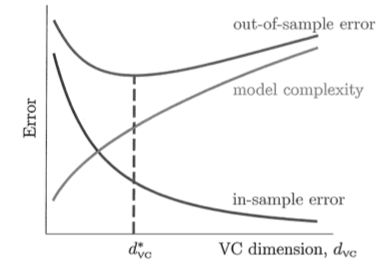
\includegraphics[scale = 0.7]{overunderfit}$$
$d^*_{vc}$ is the degree of freedom that gives the optimal model when new data is added. The out of sample error is minimalized. To the left of it, there is underfit and to the right of it, there is overfit. \\
In-Sample error: $SSE$ and $S_e$ is calculated from $\mathcal{D}$. \\
Out-of-Sample (oos) error: $oosSSE$ and $oosS_e$ are computed from future data or $\mathcal{D}^*$. \\~\\
In-sample error can go to zero since all data is already there and matched. There is no learning of $f(x)$ or $h^*(x)$. In-sample metrics are not honest. Accountibility can be received by validation from new data not in $\mathcal{D}$, never seen by $\mathcal{A}$ where the $y_i$'s are known so that it can be compared to $\hat{y}_i$'s from $g$. How do we do this if $\mathcal{D}$ is all we got? \\
Split $\mathcal{D} = \mathcal{D}_{\text{train}} \bigcup \mathcal{D}_{\text{test}}$ randomly. Select a $k$ where $\frac{1}{k}$ = the proportion of $\mathcal{D}$ in $\mathcal{D}_{\text{test}}$. Typical splits are $90\%$ train and $10\%$ test ($k = 10$) or $80\%$ train and $20\%$ test ($k = 5$). Use $g = \mathcal{A}(\mathcal{D}_{\text{train}}, \mathcal{H})$ and use $\mathcal{D}_{\text{test}}$ to predict oos. 
$$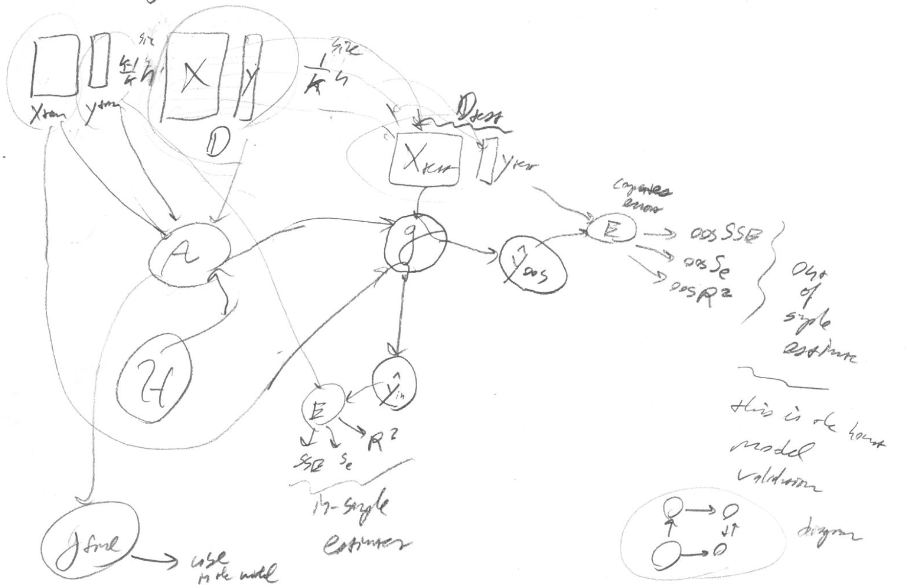
\includegraphics[width = \textwidth]{splittingdata}$$ 
In order for the oss error estimates to be honest, $\mathcal{D}_{\text{test}}$ can not be looked at until $g$ is fully constructed. It can be used only one to get oos estimates and can never be looked at again. \\~\\
Consider $h^*(x)$, a linear fit, where $\mathcal{H} = \set{w_0 + w_1x}$ with 2 degrees of freedom. This is underfitting because there is not enough degrees of freedom. There is misspecification error. $f(x)$ is parabolic. We need to make $\mathcal{H}$ richer by adding more terms beyond the linear terms. \\ 
Consider the Weierstrass Approximation Theorem: for every continuous function, $x$ in region $\in [a,b]$, there exists a polynomial function $p(x)$ such that for all $\varepsilon$, for all $x \in X$, $\abs{f(x) - p(x)} < \varepsilon$. \\
This means that any continuous function can be approximated with a polynomial. Let's begin with polynomials of degree $2$. This is $\mathcal{H} = \set{w_0 + w_1x + w_2x^2: \vec{w} \in \mathbb{R}}$. Let $X = \begin{bmatrix} x_{11} \\ \dots \\ x_{1n} \end{bmatrix}$. Here $p=1$. Add a single degree of freedom; then $X = \begin{bmatrix} 1 & x_{11} \\ \vdots & \vdots \\ 1 & x_{1n} \end{bmatrix}$. Here $p+1 = 2$ and is full rank. Now add polynomial degree of freedom. Then $$X = \begin{bmatrix} 1 & x_{11} & x_{11}^2 \\ \vdots & \vdots & \vdots \\ 1 & x_{1n} & x_{1n}^2 \end{bmatrix} $$ Here $p+1 = 3$ and is full rank. From here, use least squares are usual. This is why it's usually called a linear non-linear mode. Then $\vec{b} = (X^TX)^{-1}X^T\vec{y}$. What we'll find is $h^*(x) \approx f(x)$, or closer than before. \\
This can get improved; use polynomials of degree $3$. 
$$ X = \begin{bmatrix} 1 & x_{11} & x_{11}^2 & x_{11}^3 \\ \vdots & \vdots & \vdots & \vdots \\ 1 & x_{1n} & x_{1n}^2 & x_{1n}^3 \end{bmatrix} $$ 
If $n$ is large, the $x^3$ predictions would function as one nonsense predictor, but not so bad. What about when we have many polynomial terms? It gets really bad, especially for values between 2 consecutive data points. \\
Let $n=5$ and $df = 4$. $$ \begin{bmatrix} 1 & x_1 & x_1^2 & x_1^3 & x_1^4 \\ 1 & x_2 & x_2^2 & x_2^3 & x_2^4 \\ \vdots & \vdots & \vdots & \vdots & \vdots \\ 1 & x_5 & x_5^2 & x_5^3 & x_5^4 \end{bmatrix} \begin{bmatrix} b_0 \\ b_1 \\ \vdots \\ b_4 \end{bmatrix} = \begin{bmatrix} y_1 \\ y_2 \\ \vdots \\ y_5 \end{bmatrix} $$ Let the four rightmost columns of the first matrix be called $X$, or the Vandermonde matrix. Is it invertible? 
$$\det[X] = \prod_{i=1}^n \prod_{j=i+1}^n x_j - x_i \neq 0 $$ 
only if all $x_i$'s are unique. Therefore yes, $n$ data points can be fit by a $n-1$ degree polynomial. \\
Instead of polynomials, could you use logs, sines/cosines, exponentials and such? Yes. 

\section{Lecture 16} 
Polynomial regression is a type of ``non-linear" linear modeling. Interactions is another type of ``non-linear" linear modeling. Consider the data with $p=2$ and hypothesis set: $$\mathcal{H} = \set{w_0 + w_1x_1 + w_2x_2 + w_3x_1x_2: \vec{w} \in \mathbb{R}^4} $$ 
How fo fit? 
$$X = \begin{bmatrix} 1 & x_{11} & x_{21} & x_{11}x_{21} \\ \vdots & \vdots & \vdots & \vdots \\ 1 & x_{1n} & x_{2n} & x_{1n}x_{2n} \end{bmatrix} $$ 
The degrees of freedom is $4$. Why would you do this? \\
If $\mathcal{H} = \set{w_0 + w_1x_1 + w_2x_2}$, this translates to $g(\vec{x}) = b_0 + b_1x_1 + b_2x_2$. The interpretation of this is, if $x_1$ increases by one unit, $\vec{y}$ increases by $b_1$ units on average regardless of the value of $x_2$. \\
Say $\mathcal{H} = \set{w_0 + w_1x_1 + w_2x_2 + w_3x_1x_2}$. This translates to $g(\vec{x}) = b_0 + b_1x_1 + b_2x_2 + b_3x_1x_2 = b_0 + x_1(b_1 + b_3x_2) + b_2x_2$. This can be interpreted as, if $x_1$ increases by one unit, then $\vec{y}$ increases by $b_1 + b_3x_2$ units. \\
Now, you're given the model more degrees of freedom to have differential slopes based on the value of the other predictors. This is more expressible. \\~\\
Given the same $X$, there are many $\mathcal{H}$'s (and $\mathcal{A}$'s) to produce different $g$'s. $$ \begin{aligned} 
g_1 &= b_0 + b_1x_2 \\ g_2 &= b_0 + b_1x_1 + b_2x_2 \\ g_3 &= b_0 + b_1\log(x_1) + b_2x_2 \\ g_4 &= b_0 + b_1x_1^2 + b_2x_2 \\ &\vdots \\ g_M &= b_0 + b_1x_1 + b_2x_2 + b_3x_1x_2 \end{aligned} $$ 
There are infinite models. 
\section{Lecture 17} 

Model Selection: one of the most fundamental questions in all of statistics (maybe over science) \\
Previously, use $\mathcal{D}_{\text{test}}$ to estimate oos error. This is a conservative honest estimate of future performance. \\
 Why not test $g_1,\dots, g_M$ by fitting them on $\mathcal{D}_{\text{train}}$ and then testing them on $\mathcal{D}_{\text{test}}$ and picking the one with the best error? You can but there is a problem. What do we use now to estimate future prediction? Why can't we use $\mathcal{D}_{\text{test}}$ again? \\
 Imagine $g_1,\dots, g_M$ where $M$ is large. Find $g_j$ such that error on $\mathcal{D}_{\text{test}}$ is near $0$ by coincidence. This is not a realistic estimate of future predictions. \\~\\
 Split $\mathcal{D}$ into 3 sections, $\mathcal{D}_{\text{train}}$, $\mathcal{D}_{\text{select}}$/$\mathcal{D}_{\text{validation}}$, and $\mathcal{D}_{\text{test}}$. \\
 Model Selection and Validation Protocol: \begin{enumerate}
 \item For each model $j \in \set{1,\dots,M}$, build $g_j = \mathcal{A}_j(\mathcal{H}_j, \mathcal{D}_{\text{train}})$. 
 \item Get error $oose_j = \text{error}(y_{\text{select}}, g_j(x_{\text{select}}))$ (usually $s_e$). 
 \item Select $j^* = \argmin{} \set{oose_1, \dots, oose_M}$. 
 \item Compute $oose_{j^*} = \text{error}(y_{\text{test}}, g_{j^*}(x_{\text{test}}))$. This is the estimate of future performance. 
 \item Repeat steps 1-4 on $\mathcal{D}$ to produce $g_{\text{final}}$. \end{enumerate} 
 This is called model selection by oos error. This is one such method. Other methods are ``analytical." They rely on statistical/probabilistic models. Examples include AIC and BIC. \\~\\
$k$-Fold Cross Validation: Randomize the order of $\mathcal{D}$ and divide it into $k$ folds (slots). Note that each observation is in $\mathcal{D}_{\text{test}}$ once - its own $K$ folds. \begin{enumerate} 
\item Fit $g_k = \mathcal{A}(\mathcal{H}, \mathcal{D}_{\text{train}, k})$.
\item Calculate $\vec{\hat{y}} = g_{VC}(x_{\text{test}, k})$. 
\item Repeat 1-2 for $1-K$ folds.
\item Concat vertically $\vec{\hat{y}} = \begin{bmatrix} \vec{\hat{y}}_1 \\ \vdots \\ \vec{\hat{y}}_k \end{bmatrix} $.
\item Compute $oose = \text{error}(\vec{y}, \vec{\hat{y}_{cv}})$ where $\vec{y}$ is the full $y$ since each observation is represented across the $k$ folds. \end{enumerate} 
Cross validation gives you a lower variance estimate of future performance. See what happens with different values of $k$. Note there is no optimal value of $k$. \\
When $k=2$, $50\%$ train, $50\%$ test. This will give the highest estimate error in $g$ and the lowest value of any oos test metric, respectively. It will give a nice estimate of error but on a model which has more estimation error. 
When $k=n$, there is lower estimate error in $g$ and high variation in oos test metric. This is called LOOCV, or leave one over cross validation. \\~\\
Bootstrap Validation: Sample $n$ rows from $\mathcal{D}$ with replacement and validate on out-of-bag, the rows not sampled. \\
Protocol: \begin{enumerate} 
\item For $g_{j, k_i, k_0} = \mathcal{A}(\mathcal{H}, \mathcal{D}_{\text{train}, k_i, k_0})$.
\item Compute $\hat{y}_{j, k_i, k_0} = g_{j, k_i, k_0}(\mathcal{D}_{\text{select}, k_i, k_o})$.
\item Repeat steps 1-2 for all models $j \in \set{1,\dots,M}$.
\item Repeat steps 1-2 for all inner folds $k_i \in \set{1,\dots,5}$.
\item Concat $\vec{\hat{y}_{j, k_0}} = \begin{bmatrix} \vec{\hat{y}_{j, 1, k_0}} \\ \vdots \\ \vec{\hat{y}_{j, 5, k_o}} \end{bmatrix}$. 
\item Select the best model $j^*_{k_0} = \argmin {oose_{j, k_0}}$. 
\item Repeat steps 1-6 for $k_0 = \set{1,\dots, 5}$. 
\item Get $\vec{\hat{y}} = \begin{bmatrix} \vec{y}_{j^*_1} \\ \vdots \\ \vec{y}_{j^*_5} \end{bmatrix} $. 
\item Estimate $oose = \text{error}(\vec{\hat{y}}, \vec{y})$. 
\item Repeat steps 1-6 to build final model $g$ without $\mathcal{D}_{\text{test}}$. \end{enumerate}

\section{Lecture 18} 
Previously, model selection was covered from 
\begin{itemize} 
\item Model 1: $g_1 = b_0 + b_1x$ from $\mathcal{A}_1, \mathcal{H}_1$
\item Model 2: $g_2 = b_0 + b_1x + b_2x^2$ from $\mathcal{A}_2. \mathcal{H}_2$
\item Model 3: $g_3 = b_0 + b_1x + b_2x^2 + b_3\log(x)$ from $\mathcal{A}_3, \mathcal{H}_3$ 
\item up to Model M: $g_M = b_0 + b_1x + b_2x^2 + b_3x^3$ from $\mathcal{A}_M, \mathcal{H}_M$ \end{itemize} 
Where these models came from was never discussed. It was just made up. How can we use $\mathcal{D}_{\text{train}}$ to generate good candidates $1, \dots, M$? For linear models, this usually done iteratively. One such algorithm is: you start with a huge number of derived predictions (polynomials, logs, interactions, etc.) and then iteratively add the ``best one." But if you add too many, you overfit! So, use $\mathcal{D}_{\text{select}}$ to stop once you see yourself start to overfit. This is called ``forward stepwise" linear modeling. \\
Two Main Problems: \begin{itemize} 
\item You still need an intelligent collection of predictions to choose from at each position, are you sure you can specify that? 
\item The model will still be linear although $y_m$ can alter the $\mathcal{A}$ to do nonlinear models. \end{itemize} 
When we specified $\mathcal{H} = \set{\vec{w} \cdot \vec{x}: \vec{w} \in \mathbb{R}^{p+1}}$, we made a ``parametric assumption,"that is, the model will be of this form which is fixed. Would it be nice if $\mathcal{H}$ can adjust flexibly and allow for more complexity if $n$ increases? This is called ``non-parametric regression." Here, the model does not take a pre-specified form but is constrained to information in the data. The data provides the model space and the model estimates. \\~\\
Classification and Regression Trees: Classification trees are where $\mathcal{Y} \subseteq \set{1,\dots, K}$ whereas regression trees are where $\mathcal{Y} \subseteq \mathbb{R}$. \\
Let $f(x)$ be a sine-line curve and we want to estimate $f(x)$. If $\mathcal{H}_1 = \set{w_0 + w_1\sin(w_2x): \vec{w} \in \mathbb{R}^3}$, we will likely do very well with $3$ parameters. As for $\mathcal{A}$, we can still use linear squares but we may need to use a numerical optimizer. If $\mathcal{H}_2 = \set{w_0 + w_1x + w_2x^2: \vec{w} \in \mathbb{R}^3}$, we would likely do very poorly with $3$ parameters. In one dimension, this is easy it pick $\mathcal{H}_1$ over $\mathcal{H}_2$. In multiple dimensions, it is very difficult. Imagine the following algorithm: $g(x)$ is a collection of constant subfunctions where each has a small interval. The union of all intervals is $\mathcal{X}$. To create better resolutions, create smaller domains. \\
If the intervals are large, you get underfiting and misspecification error because the data points will vary greatly from the constant value. If the intervals are small, you get overfitting estimation error because not enough data in each tiny interval makes a good decision about where to put the constant value. \\~\\
Let $p=2$ and $\mathcal{Y} = \mathbb{R}$. Suppose the following where $L$ is the low value and $H$ is the high value. $$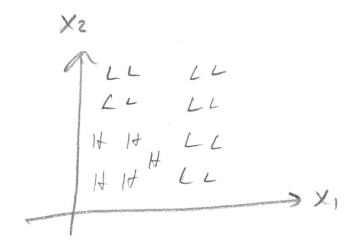
\includegraphics[width = \textwidth]{highlow}$$
What do the intervals look like in two dimensions? Shapes. It must be rectangles whose sides are parallel to the aces. What interval split makes most sense here? 
$$ 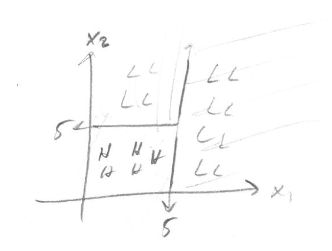
\includegraphics[width = \textwidth]{highlowlines}$$ 
This model is formed by tree intervals. 
$$ g(\vec{x}) = L\indicator{x_1 > 5} + L\indicator{x_1 \leq 5}\indicator{x_2 > 5} + H\indicator{x_1 \leq 5}\indicator{x_2 \leq 5} $$ 
It is still a linear model technically but is there another way way to visual this? Answer. Binary tree. 
$$ 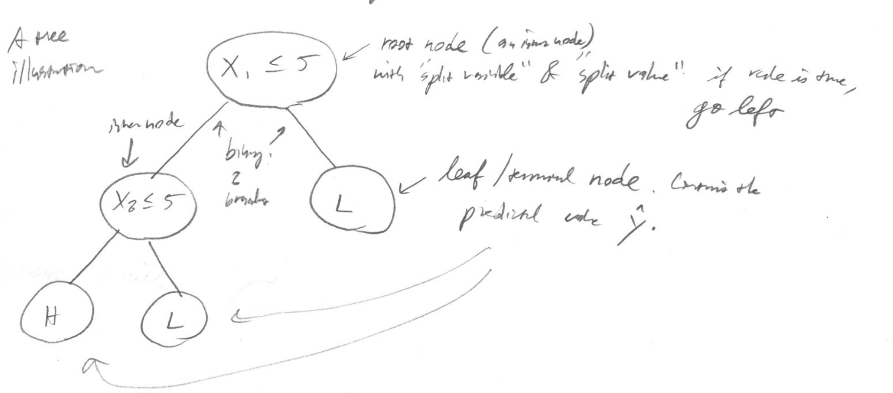
\includegraphics[width = \textwidth]{binarytree}$$ 
Is all $\mathcal{X}$ accounted for? Yes, there is a $\hat{y} ~\forall x \in \mathcal{X} = \mathbb{R}^2$. Where is the rectangle - parallel - to - axis restriction seen? Rules must be of the form ``$x_j \leq m$" which creates two rectangles parallel to the $x_j$ direction. What is $\mathcal{A}$? There are infinite possible models of this form. 

\section{Lecture 19} 
There are many ways to select splits and predictions. Here is one such algorithm. \\~\\
Binary Tree: \begin{enumerate} 
\item Begin with all training data $X,Y$. 
\item For every possible split at the current node, divide into $X_L, \vec{y}_L$ and $X_R, \vec{y}_R$ and calculate $$SSE_L = \sum (Y_L - \bar{Y}_L)^2 ~~~ SSE_R = \sum (Y_R - \bar{Y}_R)^2 $$ where the summation is done over number of data points in the split. 
\item Find the split with the lowest total SSE 
$$SSE_{tot} = SSE_L + SSE_R $$ 
\item Create the split by splitting data into two nodes. 
\item Repeat steps 2-4 until ``STOP." \end{enumerate} 
Note: STOP is when mode has less than $N_0$ data points inside. \\
If $N_0 = 14$, the tree is grown to fit a separate parameter for each data point and $R^2 = 100\%$. Then the tree is proven back to not overfit, like backwards stepwise regression. $N_0$ is picked via model selection procedure. 
\\~\\
Classification: Remember $Y = \set{0,1}$ which was binary? Now consider $Y = \set{1,2,\dots,K}$. This is $K$ groups/labels classification. What methods do we have? For binary classification, there was perceptron and SVM with hinge loss. Here $$ \begin{aligned} \mathcal{H} &= \set{\indicator{w_0 + w_1x_1 + \dots \geq 0}: \vec{w} \in \mathbb{R}^5} \\ \mathcal{A}&: \argmin{}\set{\frac{1}{n} \sum_{i=1}^n \max\set{0, \frac{1}{2} - (y_i - \frac{1}{2})(\vec{w}\vec{x}_i - b) + \lambda \norm{\vec{w}}^2}} \end{aligned} $$ 
Did we ever discuss general classification into $K > 2$ labels? No. This works using trees. \\~\\
Classification Tree Algorithm: \begin{enumerate} 
\item Begin with all training data. 
\item For every possible split, calculate the Gini impurity metrics $$ \begin{aligned} Gini_L &= \sum_{i=1}^k \hat{p}_L(1 - \hat{p}_L) \\ Gini_R &= \sum_{i=1}^k \hat{p}_R(1 - \hat{p}_R) \end{aligned} $$ where $$ \hat{p}_i = \frac{\text{number of $y_i$ in category i}}{n\text{ number in node}} $$ 
\item Find the split with the lowest weighted average of Gini impurity metric $$ Gini_{avg} = \frac{n_L Gini_L + n_R Gini_R}{n_L + n_R} $$ 
\item Create the split and split the data in the node correctly along the two new daughter nodes. 
\item Repeat steps 2-4 and ``stop." where node has $\leq N_0$ data points. (Default is $N_0 = 1$.)
\item For all leaf nodes, assign $\hat{y} = \text{Mode}[\vec{y}_0]$ where $\hat{y}_0$ is the average of the $y_i$'s in the leaf node. \end{enumerate} 

\section{Lecture 20} 
We measured error in binary classification using $MAE = \frac{1}{n}\sum_{i=1}^n \indicator{\hat{y}_i \neq y_i}$, or misclassification error. Does this work for both in-sample and out of sample? Yes. But this hides a lot of what's going on. There are two types of errors. One is, saying a true 0 is a 1, false positive (FP), and, saying a true 1 is a 0, false negative (FN). This can be visualized in a Confusion Table. $$ \begin{tabular}{lllll}
  & 0    & 1    &     &  \\
0 & TN   & FP   & \#N &  \\
0 & FN   & TP   & \#P &  \\
  & \#PN & \#PP & n   & 
\end{tabular} $$ where the $x$ axes represent the prediction ($\hat{y}$) and the $y$ axes represent the truth ($y$). PN is predicted negatives and PP is predicted positives. The rightmost column represents the number of negatives, positives, and total respectively. \\
Metrics: $$ \begin{aligned} \text{Misclassification Error} &= \frac{FP + FN}{n} \\ \text{Accuracy} &= 1 - \text{misclassification error} \\ &= \frac{TP + TN}{n} \\ \text{Precision} &= \frac{TP}{\#PP} \text{ what proportion of the predicted positives are truly positives?} \\ \text{Recall/Sensitivity} &= \frac{TP}{\#P} \text{ what proportion of those predicted truly positive were predicted positives?} \end{aligned} $$ 
Imagine there are 9 data points, 5 positives and 4 negatives. 2 of the positives are selected. Then precision = $\frac{2}{2} = 100\%$. But recall = $\frac{2}{5} = 40\%$. Now consider all 9 selected. Then precision = $\frac{5}{9} = 56\%$ and recall = $\frac{5}{5} = 100\%$. Both situations are bad so how to combine both metrics together? 
$$F_{\text{score}} = \frac{2}{\frac{1}{\text{Recall}} + \frac{1}{\text{Precision}}} $$ In the previous example, $$ F_{\text{score}} = \frac{2}{\frac{1}{1} + \frac{1}{.56}} = 72\%$$ 
There is also $$ \begin{aligned} \text{False Discovery Rate (FDR)} &= 1 - \text{precision} = \frac{FP}{\#PP} \\ \text{False Omission Rate (FOR)} &= \frac{FP}{\#PN} \end{aligned} $$ 
Probabilistic Classification: Let $Y = \set{0,1}$. Let it represent the random variable whose realization is $y$. Let $Y \sim \text{Bernoulli}(f_{pr}(x_1,\dots,x_p))$ for a given $\hat{x}_i = [x_{i1}, \dots, x_{ip}]$. The random variable is realized to $y_i = 1$ or $y_i = 0$. Where is the error terms $\delta, \varepsilon, e$? It is not needed in this construction. The goal is to model the probabilities. So error now are difference with the true probability function $t(z_1,\dots,z_p) = t_{pr}(z_1,\dots,_t)$. This means $$ Y~\text{Bern}(t_{pr}(z_1,\dots,z_t)) \iff Y = t(z_1,\dots,z_t) $$ 
No error means probabilities are $0$ or $1$. What is the difference between $t_{pr}(z_1,\dots,z_t)$ and $f_{pr}(x_1,\dots,x_p)$? Hopefully $f_{pr} \approx t$ but $f_{pr}$ will return some values in $(0,1)$ since the error due to ignorance will be explained as a non $0$ or $1$ probability. For example, $t(\vec{z}) = 1$ and $g_{pr}(\vec{x}) = 0.8$. This means that $g(\vec{x})$ will be correct most of the time and only $\frac{1}{5}$ on average will $\hat{y} = 0$ when $y = 1$. What is the difference between $f_{pr}$, $h^*_{pr}$ and $g_{pr}$? The values of these functions are further away from perfect $0$s and $1$s. \\
Null Model: $$g_{pr,0} = \frac{1}{n}\sum y_i = \hat{p} $$ On a graph of $\vec{x}$ vs probability, $f_{pr}$ is closer to $0$s, $1$s than $h^*_{pr}$ which is closer to $0$s and $1$ than $g_{pr}$. \\ As your model goes worse and worse, the probability estimates more further away from $0$s and $1$s to values closer to $g_{pr,0}$, the overall average. \\~\\
How do you create $g_{pr}$? \\
Let $Y_1 \sim \text{Bern}(f_{pr}(\vec{x}_1)) = (f_{pr})(\vec{x}_1)^{y_1}(1 - f_{pr}(\vec{x}_1))^{1 - y_1}$ and similarly for $Y_2,\dots, Y_n$. What is $\prob{Y_1,\dots,Y_n}$, the joint mass function? It is unknown until the dependence structure between $Y_1,\dots,Y_n$ is known. Typically, a big assumption is made, independence, which gives us $$ \begin{aligned} \prob{Y_1,\dots,Y_n} &= f_{pr}^{y_1}(1 - f_{pr}(\vec{x}_1))^{1-y_1} \dots f_{pr}(\vec{x}_n)^{y_n}(1 - f_{pr}(\vec{x}_n))^{1 - y_n} \\ &= \prod_{i=1}^n f_{pr}(\vec{x}_i)^{y_i}(1-f_{pr}(\vec{x}_i))^{1-y_i} \end{aligned} $$ 
Now, if we are trying to estimate $f_{pr}$, what the knowns? The $y_1,\dots,y_n$. So our goal now is to come up with $f_{pr}$ such that the probability $\prob{Y_1,\dots,Y_n}$, or likelihood, is maximized. But of course, $f_{pr}$ is arbitrarily complicated with interactions and nonlinearities. So let's make an assumption on candidate models. Let $\mathcal{H}$ be the set of all candidate probability functions of which $h^*_{pr}$ is the closest to $f_{pr}$. Then we use an algorithm $\mathcal{A}$ to pick $g_{pr}$ which is the best and hope it's close to $h^*_{pr}$. What can we use for $\mathcal{H}$? How about $\mathcal{H} = \set{\vec{w}\cdot \vec{x}: \vec{w} \in \mathbb{R}^{p+1}}$? No because $\vec{w} \cdot \vec{x} \in \mathbb{R}$ and probabilities are between $0$ and $1$. What about $\mathcal{H} = \set{\indicator{\vec{w} \cdot \vec{x} \geq 0}}$? Only $0$ and $1$, nothing in between. What if we wanted to keep the linear model but wanted an output in $(0,1)$? We need a link function $\phi(\vec{w} \cdot \vec{x})$ whose range is $(0,1)$ monotonically and smoothly. Meaning, if $\vec{w} \cdot \vec{x}$ went up, then so does the probability estimation. Also $\phi(\vec{w} \cdot \vec{x}) \neq 0$ nor $1$ because we can never be sure. There is always information we do not know. There are many possible $\phi$ functions, or activation functions. The most popular one is the logistic function $$ \phi(u) = \frac{e^u}{1 + e^u} = \frac{1}{1 + e^{-u}} $$ There is also the probic function $$ \phi(u) = \Phi^{-1}(u) $$ where $\Phi^{-1}$ is the inverse cdf of the standard normal distribution. There is also the complementary log-log. 
$$ \phi(u) = 1 - e^{-e^u} $$ 
Why is this in $(0,1)$? $$ \begin{aligned} e^u &\in (0,\infty) \\ -e^u &\in (-\infty,0) \\ e^{-e^u} &\in (0,1) \\ 1 - e^{-e^u} &\in (0,1) \end{aligned} $$ 
There is also the hyperbolic tangent $$ \phi(u) = \tanh(u) = \frac{e^u - e^{-u}}{u^u + e^{-u}} $$ 
Use the logistic $\phi$. Then $$ \mathcal{H} = \set{ \frac{e^{\vec{w} \cdot \vec{x}}}{1 + e^{\vec{w} \cdot \vec{x}}}: \vec{w} \in \mathbb{R}^{p+1}} $$ $\mathcal{A}$ will maximize the likelihood: 
$$\begin{aligned} \vec{b} &= \argmax{\vec{w}} \set{\prob{Y_i, \dots,Y_n}} 
\\ &= \argmax{\vec{w}} \set{\prod_{i=1}^n (\frac{e^{\vec{w} \cdot \vec{x}_i}}{1 + e^{\vec{w} \cdot \vec{x}_i}})^{y_i}(1 - \frac{e^{\vec{w} \cdot \vec{x}_i}}{1 + e^{\vec{w} \cdot \vec{x}_i}})^{1 - y_i}} 
\\ &= \argmax{\vec{w}} \set{ \prod_{i=1}^n (\frac{1}{1 + e^{-\vec{w} \cdot \vec{x}_i}})^{y_i}(\frac{1}{1+e^{\vec{w} \cdot \vec{x}_i}})^{1 - y_i}} 
\\ &= \begin{cases} (1 + e^{-\vec{w} \cdot \vec{x}_i})^{-1} &\text{ if } y_i = 1 
\\ (1 + e^{\vec{w} \cdot \vec{x}_i})^{-1} &\text{ if } y_i = 0 \end{cases} 
\\ &= (1 + e^{(1 - 2y_i)\vec{w} \cdot \vec{x}})^{-1} 
\\ &= \argmax{\vec{w}}\set{\prod_{i=1}^n (1 + e^{-z_i\vec{w} \cdot \vec{x}_i})^{-1}} 
\text{ where } z_i = 2y_i - 1 \end{aligned} $$ 
Note: If we are taking $\argmax{} \set{v(t)}$, this is equal to $\argmin{} \set{\ln(v(t))}$ since $\ln$ is a monotonic increasing transformation. Therefore $$ \vec{b} = \argmax{\vec{w}} \set{\ln(\prod_{i=1}^n (1 + e^{-z_i\vec{w} \cdot \vec{x}_i})^{-1})} = \argmax{\vec{w}}\set{-\sum_{i=1}^n \ln (1 + e^{-z_i\vec{w} \cdot \vec{x}_i})} = \argmin{\vec{w}}\set{\sum_{i=1}^n \ln(1 + e^{-z_i\vec{w}\cdot\vec{x}_i})} $$ Now differentiate with respect to $\vec{w}$ and set it equal to $0$ to solve for $\vec{b}$. No closed form. 

\section{Lecture 21} 
Let the model be $y = t(\vec{z})$. The stuff you don't know appear as $Y \sim \text{Bern}(f_{pr}(\vec{x}))$. Given he same $\vec{x}$, sometimes $y=1$ and sometimes $y = 0$. So if we care about $\prob{Y = 1| X}$, our target is $f_{pr}(\vec{x})$. But $f_{pr}(\vec{x})$ can be arbitrarily complicated so we try to approximate it using a function in $\mathcal{H}$ Let $$\mathcal{H} = \set{ \frac{e^{\vec{w} \cdot \vec{x}}}{1 + e^{\vec{w} \cdot \vec{x}}}: \vec{w} \in \mathbb{R}^{p+1}} $$ Our $\mathcal{A}$ was to maximize likelihood, assuming $Y_i$ is individual and so $$ \vec{b} = \argmin{\vec{w}} \set{\sum_{i=1}^n \ln (1 + e^{-z_i\vec{w} \cdot \vec{x}_i})} $$ where $z_i = 2y_i - 1$. This looks like $\sum e_i$. and so $e_i > 0$. If $y_i = 1$, $e_i = \ln(1 + e^{-\vec{w} \cdot \vec{x}_i})$ and so if $\vec{w} \cdot \vec{x}_i$ is positive and large, the error is small. If $\vec{w} \cdot \vec{x}_i$ is negative. If $y_i = 0$, $e_i = \ln(1 + e^{\vec{w} \cdot \vec{x}_i})$ and so if $\vec{w} \cdot \vec{x}_i$ is negative and large, the error is small. \\ Use numerical methods to solve for the derivative of $\sum e_i = 0$. \\~\\
Let $$ \hat{P}_i^* = g(\vec{x}^*) = (1 + e^{-\vec{b} \cdot \vec{x}^*})^{-1} = \hat{P}(Y_i = 1 | \vec{X}_i) $$ This is the probability estimate for new $\vec{x}^*$. The linear term $\vec{b} \cdot \vec{x}$ is buried inside. Does it have meaning? $$ 1 - \vec{p} = (1 + e^{\vec{b} \cdot \vec{x}^*})^{-1} = \prob{Y_i = 0 | \vec{X}_i})$$ Now define odds as $$ \frac{\hat{p}}{1 - \hat{p}} = \frac{1 + e^{\vec{b} \cdot \vec{x}}}{1 + e^{-\vec{b} \cdot \vec{x}}} = e^{\vec{b} \cdot \vec{x}} $$ Then $$ \ln \frac{\hat{p}}{1-\vec{p}} = \vec{b} \cdot \vec{x} $$ This is the log-odds of $Y | \vec{X}$. If it is very negative, there is a low probability. If is it very positive, there is a high probability. If it is near zero, it has $50\%$ probability. \\~\\
Validating Probability Models: What is the best probability model you can make? $f_{pr}$. So we should validate against $f_{pr}$. But we can't and so we have to validate $\vec{p}$ against $\vec{y}$. This brings up the theory of scoring functions or scoring rules. \\ Let $S(\vec{p}_i, y_i)$ be the scoring rule for observations. A proper scoring rule has the following property: for all $i$, $$f_{pr}(\vec{x}_i) = \argmax{\hat{p}} \set{S(\hat{p}, y_i)} $$ The expected scoring value is maximized if you use the true probability. Popular scoring rules are the log scoring rule: $$ S_i = y_I\ln(\hat{p}_i) + (1-y_i)\ln(1-\hat{p}_i) $$ If $y_i = 1$, this is almost zero when $\hat{p} \approx 1$. If $y_i = 0$, this is almost zero when $\hat{p} \approx 0$. The log scoring rule is evaluated on $$ \text{avg score} = \frac{1}{n} \sum_{i=1}^n S_i$$ The Brier score is $$S_i = -(y_i - \hat{p}_i)^2 $$ 
Does the average score mean anything in the problem? No, it is just a means to validate and compare models. To validate, you need to think in Brier scores. What's another way to validate? Use probability estimation to do classification and then validate the classification. \\
How to turn a $\hat{p}$ into a $\hat{y}$? Use the probability model to do binary classification. \\ 
If $Y$ is predicted to be $1$, with probability $90\%$, $\hat{y} = 1$. If it has probability $10\%$, $\hat{y} = 0$. If it it has probability $51\%$, $\hat{y} = 1$. This is the hard threshold rule $$ \hat{y}_i = \indicator{\hat{p}_i \geq 0.5} $$ 
What if you do it $\hat{y}_i = \indicator{\hat{p}_i \geq 0.9}$? This makes it very difficult to get $\hat{y}_i = 1$. This means you are being very conservative to predict a $1$. What happens to the confusion table? FP goes up and FN goes down. You are saying the cost of FP is greater than the cost of FN. This is the idea of asymmetric cost classifiers/models. \\~\\
Generally, $$\hat{y}_i = \indicator{\hat{p}_i \geq p_{th}} $$ where $th$ is the threshold. Obviously, $p_{th} \in (0,1)$. One probability model can lead to infinite classification models since each value of $p_{th}$ gives a new classifier. Why not look at all of them? \\
Make a table of $p_{th}$, TP, TN, FP, FN, precision, recall, FDR, FOR and FPR, for $p_{th}$ from $0.01$ to $0.99$. Now plot a performance curve of all possible models. One example is the receiver operating characteristic curve (ROC). This is a graph of false positive rate (FPR) on the x axis vs recall on the y axis, both from 0 to 1. The line of random guessing is the y=x line. The plot of model performance is a curve from (0,0) to (1.1) outwards from the line of random guessing. The best model will have no error and be close to (0,1). Now, consider the area under the curve, AUC. If it is greater than 0.5, then the majority of models performed better than chance. \\
Consider the case where if you use the null models, you classify positives with probabilities $p_{th}$. The null models is $Y \sim \text{Bern}(p_{th})$ where $p_{th} \in (0,1)$. If $p_y$ is $\prob{Y=1}$, the marginal base rate, then the following is the confusion table. $$ 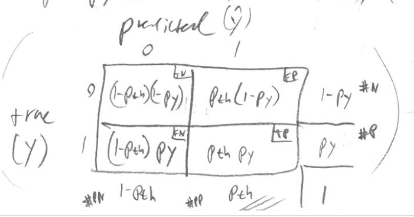
\includegraphics[width = \textwidth]{newct} $$ 
Then $$FPR = \frac{FP}{N} = \frac{p_{th}(1-p_y)n}{1-p_y} = p_{th} $$ and $$ \text{recall} = \frac{TP}{\#P} = \frac{p_{th}p_yn}{p_yn} = p_{th} $$ 

\section{Lecture 22} 
This is the most popular illustration of model options, detection error tradeoff (DET). Plot miss rate (FN / P) versus FDR = FP / PP . This is a inward looking curve where (0,0) is the point of perfection and (0.5,1) is the point of null model. Under the null model, $$FDR = \frac{p_{th}(1-p_y)n}{p_{th}n} = 1 - p_y $$ and $$\text{miss rate} = \frac{(1-p_{th})p_yn}{p_yn} = 1 - p_{th} $$ As FP goes up, FN goes down. If $p_{th} = 0$, then all $\hat{y}_i = 1$ and never misses anything. If $p_{th} = 1$, then all $\hat{y}_i = 0$ and misses everything and FDR is undefined. \\~\\
How to select a classifier? One point on the ROC or DET plot. You need to define your costs and rewards. 
$$\text{average cost} = \frac{1}{n}(c_{FP}FP + c_{FN}FN) $$ where $c_{FP}$ is the cost of FP and $c_{FN}$ is the cost of FN. Also, $$ \text{average reward} = \frac{1}{n}(-c_{FP}FP + r_{TP}TP - c_{FN}FN + r_{TN}TN) $$ Imagine you are trying to send people a mailing advertiser to open a credit card and the mail costs $\$5$. The TP is you mail to a person who opens the new credit card. Then $r_{TP} = 1000 - 5$. TN is you don't mail to a person who does not open a card. Then $r_{TN} = 0$. FP is you mail to a person but they don't open a credit card, then $c_{FP} = 5$. FN is you don't mail to someone who would open the card, then $c_{FN} = 1000$. So you want to build a model where FN is minimized. Don't worry about FP as much. Keep $p_{th}$ small. \\~\\
Bias-Variance Decomposition: Recall that $$y = g+ e = g+ (f-g) + \delta$$ where $f-g$ is the error due to misspecification and estimator and $\delta$ is the error due to ignorance. Then $$ e = y -g = f-g+\delta$$ $e=f-g$ is the measure of how good the model $g$ is. Then $$e^2 = (f-g+\delta)^2$$ 
What if I wanted the mean squared error MSE? This is the expectation of the squared residuals. In order to take an expectation, you need random variables. \\
Let $Y = f(\vec{x}) + \Delta$ where $Y$ is a random variable for response and $\Delta$ is a random variable for error. Now suppose $$ Y | \vec{X} = \vec{x} = f(\vec{x}) + \Delta | \vec{X} = \vec{x} $$ Assume $\expe{Y | \vec{X} = \vec{x}} = f(\vec{x})$, this is the conditional expectation function. Then $\expe{\Delta |\vec{X} = \vec{x}}=0$. So for any $\vec{x}$, the average of the $y$s that were realized are close to $f(\vec{x})$. Assume also that variance does not depend on $\vec{x}$, or the homoscedastic assumption, or $\var{\Delta | \vec{X} = \vec{x}} = \var{\Delta} = \sigma^2$. Hence $\expe{\Delta^2} = 0$. Now, back to MSE. We care about this for a new observation $\vec{x}^*$. This is also called generalization error. Then $$ MSE(\vec{x}^*) = \expe{(Y^* - g(\vec{x}^*))^2 | \vec{X} = \vec{x}^*} \geq \sigma^2 $$ It cannot be better than the irreducible error. What if we know $f$? $$ MSE(\vec{x}^*) = \expe{(Y^* - f(\vec{x}^*))^2 | \vec{X} = \vec{x}^*} = \expe{\Delta^{*2} | \vec{X} = \vec{x^*}} = \expe{\Delta^{*2}} = \sigma^2 $$ What is this expectation over? It is over $\Delta^*$, an integral over $\mathbb{R}$ with $\prob{\Delta}$ inside. \\
If $f$ is unknown, $$ \begin{aligned} MSE(\vec{x}^*) & = \expe{Y^{*2} - 2Y^*g(\vec{x}^*) + g(\vec{x}^*)^2 | \vec{X} = \vec{x}^*} \\ &= \expe{Y^{*2} | \vec{X} = \vec{x}^*} - 2\expe{Y^*g(\vec{x}^*) | \vec{X} = \vec{x}} + \expe{g(\vec{x})^2 | \vec{X} = \vec{x}^*} \\ &= \expe{(f(\vec{x}) + \Delta)^2 | \vec{X} = \vec{x}^*} - 2\expe{Y^*}g(\vec{x}^*) + g(\vec{x})^2 \\ &= \expe{(f(\vec{x}) + \Delta)^2} - 2f(\vec{x}^*)g(\vec{x}) + g(\vec{x})^2 \\ &= \expe{f(\vec{x}^*)^2 + 2f(\vec{x}^*)\Delta + \Delta^2} + f(\vec{x}^*)g(\vec{x}) + g(\vec{x})^2 \\ &= (f(\vec{x}^*) - g(\vec{x}^*))^2 + \sigma^2 \end{aligned} $$ 
Now since expected squared errors are additive, $e = (f-g)+\delta$, take the expectation over all $\Delta_i$ and $\Delta^*$, or expectation over all $\mathcal{D}$. Then 
$$ \begin{aligned} MSE(\vec{x}^*) &= \mathrm{E}_{\Delta_1,\dots,\Delta_n,\Delta^*}[Y^{*2} | \vec{X} = \vec{x}^*] - 2\mathrm{E}_{\Delta_1,\dots,\Delta_n,\Delta^*}[Y^*g(\vec{x}^*) | \vec{X} = \vec{x}^*] + \mathrm{E}_{\Delta_1,\dots,\Delta_n, \Delta^*}[g(\vec{x}^*)^2 | \vec{X} = \vec{x}^*] \\ &= \mathrm{E}_{\Delta^*}[Y^{*2} | \vec{X} = \vec{x}^*] - 2\mathrm{E}_{\Delta_1,\dots,\Delta_n,\Delta^*}[Y^*(g(\vec{x}^*)) | \vec{X} = \vec{x}^*] + \mathrm{E}_{\Delta_1,\dots,\Delta_n}[g(\vec{x}^*)^2] \\ &= \sigma^2 + f(\vec{x}^*)^2 - 2\mathrm{E}_{\Delta^*}[Y^*]\mathrm{E}_{\Delta_1,\dots,\Delta_n}[g(\vec{x}^*)] + \mathrm{E}_{\Delta_1,\dots,\Delta_n}[g(\vec{x}^*)^2] \\ &= \sigma^2 + f(\vec{x}^*)^2 - 2f(\vec{x}^*)\expe{g(\vec{x}^*)} + \var{g(\vec{x}^*)} + \expe{g(\vec{x}^*)}^2 \\ &= \sigma^2 + \var{g(\vec{x}^*)} + (\expe{g(\vec{x}^*)} - f(\vec{x}^*))^2 \\ &= \sigma^2 + \var{g(\vec{x}^*)} + \expe{g(\vec{x}^*) - f(\vec{x}^*)}^2 \end{aligned} $$ 
The variance term is $\expe{(g(\vec{x}) - \expe{\vec{x}})^2}$, or how much $g$ varies around its mean function $\expe{g(\vec{x})}$. The expectation term is bias, or Bias$[g(\vec{x})]^2$. It tells how far away the average $g$ is from $f$. This is the bias-variance tradeoff. This was all for one data point $\vec{x}^*$. We can average over all $\vec{x}_1,\dots,\vec{x}_n,\vec{x}^* \in X$. Assume the distribution is $\prob{\vec{X}}$. Then the general error MSE is $$ \begin{aligned} \mathrm{E}_X[\sigma^2 + \var{g(\vec{x}^*)} + \text{Bias}[g(\vec{x})]^2] \\ &= \sigma^2 + \underbrace{\mathrm{E}_X[\var{g(\vec{x}^*)}]}_{\text{expected variance}} + \underbrace{\mathrm{E}_X[\text{Bias}[g(\vec{x}^*)]^2]}_{\text{expected bias}^2} \end{aligned} $$ 


\section{Lecture 23} 

We know that $$ Y | \vec{X} = \vec{x} = g(\vec{x}) + (h^*(\vec{x}) - g(\vec{x})) + (f(\vec{x}) - h^*(\vec{x})) + \Delta $$ 
Then $$ \expe{(Y - g(\vec{x}) | \vec{X})^2} = \expe{(h^*(\vec{x}) - g(\vec{x})) + (f(\vec{x} - h^*(\vec{x})) + \Delta)^2} $$ Now $$ \begin{aligned} MSE &= \expe{\underbrace{(h^* - g)}_{V}^2 - (\underbrace{f-h^*}^B)^2 + \Delta^2 + 2(\underbrace{h^*-g}_{V})\Delta + 2(\underbrace{f-h^*}_{B})\Delta + 2(\underbrace{h^*-g}_{V})(\underbrace{f-h^*}_{B})} \\ &= \expe{V^2} + B^2 + \sigma^2 + 2B\expe{V} \\ &= \var{V} + B^2 + \sigma^2 + 2B\expe{V} + \expe{V}^2 \end{aligned} $$ 
If the algorithm is unbiased in the estimate of $g$, then $\expe{V} = 0$, such as in OLS. If the algorithm is unbiased, $$ MSE = \expe{\var{g-h^*}} + \expe{\text{Bias}[h^*]^2} + \sigma^2 $$ where the first term is estimation error component, the second term is misspecification error component and the last term is irreducible error component. Now if $n \to \infty$, $g \to h^*$, so estimation error goes to $0$. But the bias will always be the same. \\~\\
How to minimize bias? Make $h^* \to f$ by increasing model complexity. Is there a tradeoff? Yes and no. The tradeoff is between underfitting (high bias and low variance) and overfitting (low bias and high variance). Perfect fitting minimizes both. $$ 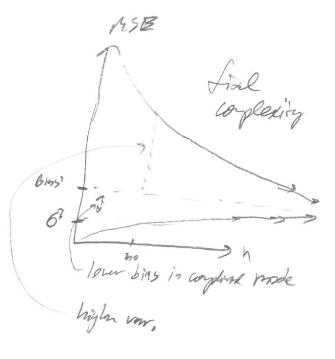
\includegraphics[width = \textwidth]{biasplot} $$ 
Regression trees have low bias because it has the ability to get close to complicated $f$ and high variance between they tend to overfit. \\~\\
Note that when many models are averaged together, it is very stable. Consider the average model as a model itself $$ g_{\text{avg}} = \frac{g_1 + \dots + g_M}{M} $$ The average of many trees is very low in bias. Can we average many trees together? With one tree, it is deterministic. So we can't, unless we change $\mathcal{D}$ or change $\mathcal{A}$ to be random. What if we change $\mathcal{D}$? Let's sample $n$ rows from $\mathcal{D}$ with replacement. This is called a bootstrap sample. This $\mathcal{D}_1$ is $\approx \mathcal{D}$ but is a little bit different. It has about $\frac{2}{3}$ of the original rows and perhaps even duplicates. So let's fit $g_1 = \mathcal{A}(\mathcal{H}, \mathcal{D}_{1})$ using regression trees. Now draw another bootstrap sample $\mathcal{D}_2$ and build another tree $g_2 = \mathcal{A}(\mathcal{H}, \mathcal{D}_2)$, and so forth. Then $g_1,\dots,g_B$ are all regression trees which are similar. Then $g_{\text{avg}}$ is the average or aggregate tree. The combination of bootstrap and aggregation is called Bagging. It is also called the meta-algorithm which leads to improvements for unstable procedures (such as high variance algorithms). \\ 
Imagine a tree $g_t$. It has low bias and high variance. Many trees averaged is $$g_{\text{bagged}} = \frac{g_1 + \dots + g_T}{T} $$ It has low bias since $$ \begin{aligned} \text{Bias} &= \expe{g_{\text{bagged}}} - f \\ &= \expe{\frac{g_1 + \dots + g_T}{T}} - f \\ &= \frac{1}{T} \expe{g_1 + \dots + g_T} - \frac{Tf}{T} \\ &= \frac{1}{T}(\expe{g_1 - f + g_2 - f + \dots + g_T - f}) \\ &= \frac{1}{T}((\expe{g_1} - f) + (\expe{g_2} - f) + \dots + (\expe{g_T} - f)) \\ &= \frac{T}{T} \end{aligned} $$ where $\expe{g_i} - f$ is the bias of the $i$th tree (small). But the variance term looks like $$ \begin{aligned} \var{g_{\text{bagged}}} &= \var{\frac{g_1 + \dots + g_T}{T}} \\ &= \frac{1}{T^2} \var{\sum g_t} \\ &\frac{1}{T^2} \sum \var{g_i} \text{ if trees are independent} \\ &= \frac{\var{g_i}}{T} \end{aligned} $$ which means as number of trees $T \to \infty$, the variance term disappears. Therefore $$ MSE = \sigma^2 + \frac{\var{g_i}}{T} + \text{Bias} \approx \sigma^2 $$ 
What is the problem with this? $g_1,\dots,g_T$ are not actually independent because usually from the same data (bootstrap samples) But if they are from different data, this works. As long as $n_t$ is large enough to create an unbiased model, then your MSE will be very small. Usually, you use all of $\mathcal{D}$ to build $g_{\text{bagged}}$ in which case the trees are dependent because bootstrap samples contains a lot of the same data. \\~\\
If $X_1,\dots,X_n$ are identically distributed but not independent, $$ \begin{aligned} \var{\bar{X}_n} &= \var{\frac{1}{n} \sum X_i} \\ &= \frac{1}{n^2} (\var{X_1} + \dots + \var{X_n} + \sum_{i\neq j} \mathrm{Cov}[X_i,X_j]) \\ &= \frac{1}{n^2}(n\sigma^2 + (n^2 -n)\sigma_{ij}) \\ &= \frac{1}{n}(\sigma^2 + (n-1)\sigma_{ij}) \\ &= \frac{1}{n}(\sigma^2 + (n-1)\rho\sigma^2) \text{ where } \rho_{ij} = \frac{\sigma_{ij}}{\sigma_i\sigma_j} = \frac{\sigma_{ij}}{\sigma^2} \\ &= \frac{1}{n}(n\rho\sigma^2 + \sigma^2 - \rho\sigma^2) \\ &= \rho\sigma^2 + \frac{1-\rho}{n}\sigma^2 \end{aligned} $$ Note that as $\rho \to 0$, $\var{\bar{X}} = \frac{\sigma^2}{n}$. Now $$ MSE = \sigma^2 + (\rho\var{g_t} + \frac{1-\rho}{T}\var{g_T}) + \text{Bias}[g_t]^2 $$ where the middle term is the variance term is an strictly less than $\var{g_t}$ itself since $\rho \neq 1$. This is why bagging works so well. \\~\\
Validation for Bagged Models (not only trees): Usually $\mathcal{D} = \mathcal{D}_{\text{train}} \bigcup \mathcal{D}_{\text{test}}$ where we build on train and validate on test. Here, each tree has its own $\mathcal{D}_{\text{train}, t}$ and $\mathcal{D}_{\text{test}, t}$ (usually called out of bag). Now we do bootstrap sample, meaning that each tree can validate itself by predicting on $\mathcal{D}_{\text{test}, t}$. Now, let each tree do so and average by observation. \\ Suppose there are $n$ observations, Observation $1$ was it was seen on tree $1$ and $5$,, observation $2$ on tree $2$ and $4$, and so on. Then validate the first observation by having it on trees $1$ and $5$ and averaging the $\hat{y}s$. Validation for the second observation is done on trees $2$ and $4$ and the $\hat{y}$s are averaged, and so forth. If $T$ is sufficiently large, all $n$ observations will be validated. We then compute $e_i$s and then an error metric such as $R^2_{oos}$, $s_{e,oos}$, etc. Now, out of bag error estimation will work. Theoretically it is like $k$-fold cross validation with $k=2$. 

\section{Lecture 24}
Why does bagging trees work so well? \begin{itemize} 
\item No need to specify a model (or do model selection) since trees figure out the model for you 
\item No need to specify hyperparameters; pick a low $N_0$
\item You get validation for free, no need to do $k$-fold CV 
\end{itemize} 
Can we do better? $$ MSE = \sigma^2 + \rho \var{g_t} + \frac{1-\rho}{T}\var{g_t} + \text{Bias}[g_t]^2 $$ 
If we can make $\rho$ as low as possible, then the variance term can be minimized. $\rho$ is the average correlation between the trees' $\hat{y}$s. How can we decorrelate the trees? Use the classification/regression tree algorithm. How about at each split, pick a random subset of features $$ \set{1,2,\dots,p_{try}} \in \set{1,2,\dots,p}$$ and then minimize SSE as usual. By doing this, each $g_t$ now is different. The bias of $g_t$ goes but not so much. Each tree is random. Together, it's called a random forest. \\~\\
For regression, $y = t(z_1,\dots,z_t)$ where $z_1,\dots,z_t$ are said to be immediate causal factors of the phenomenon $y$. They occur before $y$. This is not so clear. We don't in general see the $z$'s in the our data but we do see $x$'s. In one scenario, an $x$ could be disconnected from $y$ and $z$s; this is a bad model since there is no connection. Another scenario could be where $x$ affects only one $z$ where multiple $z$s affect $y$. This means an $x$ can be causal but not definite. A third scenario is where $x$ is affected by $z_1$ and $z_1,\dots,z_p$ affect $y$. Here, instead of a cause, it can be an incidental effect of an actual cause. Let's assume $n$ is very large. Then $x$ has a correlation with $y$ for scenario $2$ and $3$ but not $1$. Now if $n$ is moderate, then correlation could be a maybe. In the first one, it could be by random chance; in the second and third one, it could be too weak to detect. In fact, correlation in $1$ is called a spurious correlation because $x$ is divorced from causal chain. It only appears to be correlated with $y$ due to random chance. But what happens when you get more data? It disappears. What happens when you get more data for $2$ and $3$? You will see more correlation. In conclusion, is correlation causation? In scenario $1$, no because there's no correlation. In $2$, yes because it is remote from the immediate effects but it is real. In $3$, no because it itself is an effect. Now, what must be present to call a variable causal? An ability to manipulate it and see a change in $y$. Assume $x$ and $y$ are related to a certain $z$. If you manipulate $x$, does $y$ change? For example, if $x$ is number of umbrellas sold and $y$ is car accidents, are $x$ and $y$ correlated? Yes. If $x$ changes, then $y$ changes. In fact, $x$ and $y$ are correlated through the common cause $z$, which is rainfall amount. 

\section{Lecture 25} 
In scenario A, let $z$ and $y$ be connected and $x$ separated from the two. Then there is no correlation nor causation. In scenario B, let $y$ be connected to all the $z$s which are linked to other factors, one of which being $x$. Then there is correlation and causation. In scenario C, suppose $z$ is linked to $x$ and $y$ but $x$ and $y$ are not linked to each other. Then there is correlation but no causation. \\
Causality means that if you manipulate $X$ (and nothing else), you will see a change in $Y$. Which variables are the causals? The ones you don't see, the $u$s. Suppose in scenario C, $x$ is the number of umbrella sold by noon, $y$ is the number of car accidents from $12$am to $11:59$pm and $z$ is the precipitation for the day. Then $z$ is the unobserved common cause. It is also called a lurking variable because it is unobserved and affects the relationship between $x$ and $y$ when accounted for. \\~\\
Linear Model: After the OLS algorithm, $$ g(z) = b_0 + b_1x$$ What is the interpretation of $b_1$. ``If $x$ is increased by one unit on its measurement scale, then $y$ is predicted to increase by $b_1$  units on average on its measurement scale, assuming the linear model option for least squares.'' Change this to: ``When comparing two observations A and B sampled in the same way as the data in $\mathcal{D}$, where A has an $x$ value one unit larger than the $x$ value of B, then A is predicted to have a response $y_A$ that differs by $b_1$ on average from $y_B$ assuming the linear model.'' \\~\\
Can you say, ``If I increase the $x$ value for the observation, its predicted response will increase by $b_1$, assuming the linear model?" Note: This is a causal situation. Therefore you cannot usually say this unless you know it is causal. There is no way to prove when $x$ falls int he causal chain without more work. The gold standard to be able to make a causal claim is the randomized controlled experiment. \\~\\
Nonlinear Linear Models: Suppose $$g(\vec{x}) = b_0 + b_1x_1 + \dots + b_px_p $$ 
What is the interpretation of $b_1$? \\
``When comparing two observations A and B sampled in the same way as the data in $\mathcal{D}$ where A has an $x_1$ value one unit higher than B and all other $x_j$s are exactly the same, A is predicted to have a response $y_A$ that differs from $y_B$ by $b_1$ on average assuming the linear model optimal for least squares." \\~\\
A new thing wrong with this: Imagine $X_1$ is overall GPA and $X_2$ is major GPA. Can you increase $X_1$ keeping $X_2$ constant? Yes but it is weird since $X_1$ and $X_2$ are highly correlated. Ao you can make the statement about $b_1$ but it may not even be a realistic statement because A and/or B may not be observable in the real world. \\
Here's where correlation does not imply causation. Look at scenario C. Let $ y \sim x$, or $y = b_0 + b_1x$. You see an effect and $b_1$ is positive of $x$ on $y$. Now suppose $y \sim x + z$, or $y = b_0 + b_1x + b_2z$. Here you do not see an effect and $b_1$ never has a zero effect of $x$ on $y$. What is the interpretation of $b_1$? ``If $z$ stays constant (?) and $x$ changes, then $y$ doesn't change" This is contradictory to the diagram. $z$ causes $y$ and manipulating $x$ does not have any effect on $y$. \\~\\

Inference for Linear Models: Let $y = h^*(\vec{x}) + \varepsilon$. In the linear model case, $\mathcal{H} = \set{\vec{w} \cdot \vec{x}: \vec{w} \in \mathbb{R}^{p+1}}$. Then $$y = \beta_0 + \beta_1x_1 + \dots + \beta_px_p + \varepsilon $$ where $\beta$s are the true best weights and $$y = g(\vec{x}) + e = b_0 + b_1x_1 + \dots + b_px_p$$ We want to see how close $b_i$s are to $\beta_j$s and be able to test if $\beta_j = 0$. First, make the four linear regression assumptions: \begin{itemize} 
\item $h^* = f$ - that is, the true model is linear 
\item Independence of epsilons 
\item Normality of epsilons 
\item Homoscedastic of epsilons \end{itemize}
The last $3$ can be summarized as $$ \varepsilon_1,\dots,\varepsilon_n \stackrel{iid}{\sim} N(0, \sigma^2) $$ 
Theorems: \begin{enumerate} 
\item $\var{\vec{b}} = \sigma^2(X^TX)^{-1}$ 
\item $\frac{b_j}{s_{b_j}} \sim T_{n - (p+1)} $ where $T$ is the Student's T distribution; this allows for t-tests for $H_0: \beta_j = 0$, or determining if $x_j$ does not affect $y$ linearly
\item $\frac{ \frac{SSR}{(p+1)-1}}{\frac{SSE}{n-(p+1)}} \sim F_{p+1, n-(p+1)}$ where $F$ is the Fisher's F distribution; this allows for F-tests for $H_0: \forall b_j = 0$, or determining of any variables affect $y$ linearly
\item $\frac{\frac{\Delta SSR}{\Delta p}}{\frac{SSE_{full}}{n - (p+1)}} \sim F_{\Delta p, n - (p+1)}$ where $\Delta SSR$ is between a full model and a partial model; this allows for F tests for $H_0: \beta_j = 0$ and $\beta_k = 0$ and so on as per your choosing, or determining if there is any significance in a collection of variables 
\item $\hat{Y}^* \approx N(\vec{x}^*\vec{b}, \text{RMSE}^2)$ - determines empirical value for new $y^*$ and the error related to it \end{enumerate} 











\end{document}